\FloatBarrier
\clearpage
\section{Additional checks}
\label{appendix:pileup_checks}

\begin{figure}[htb!]
\centering
{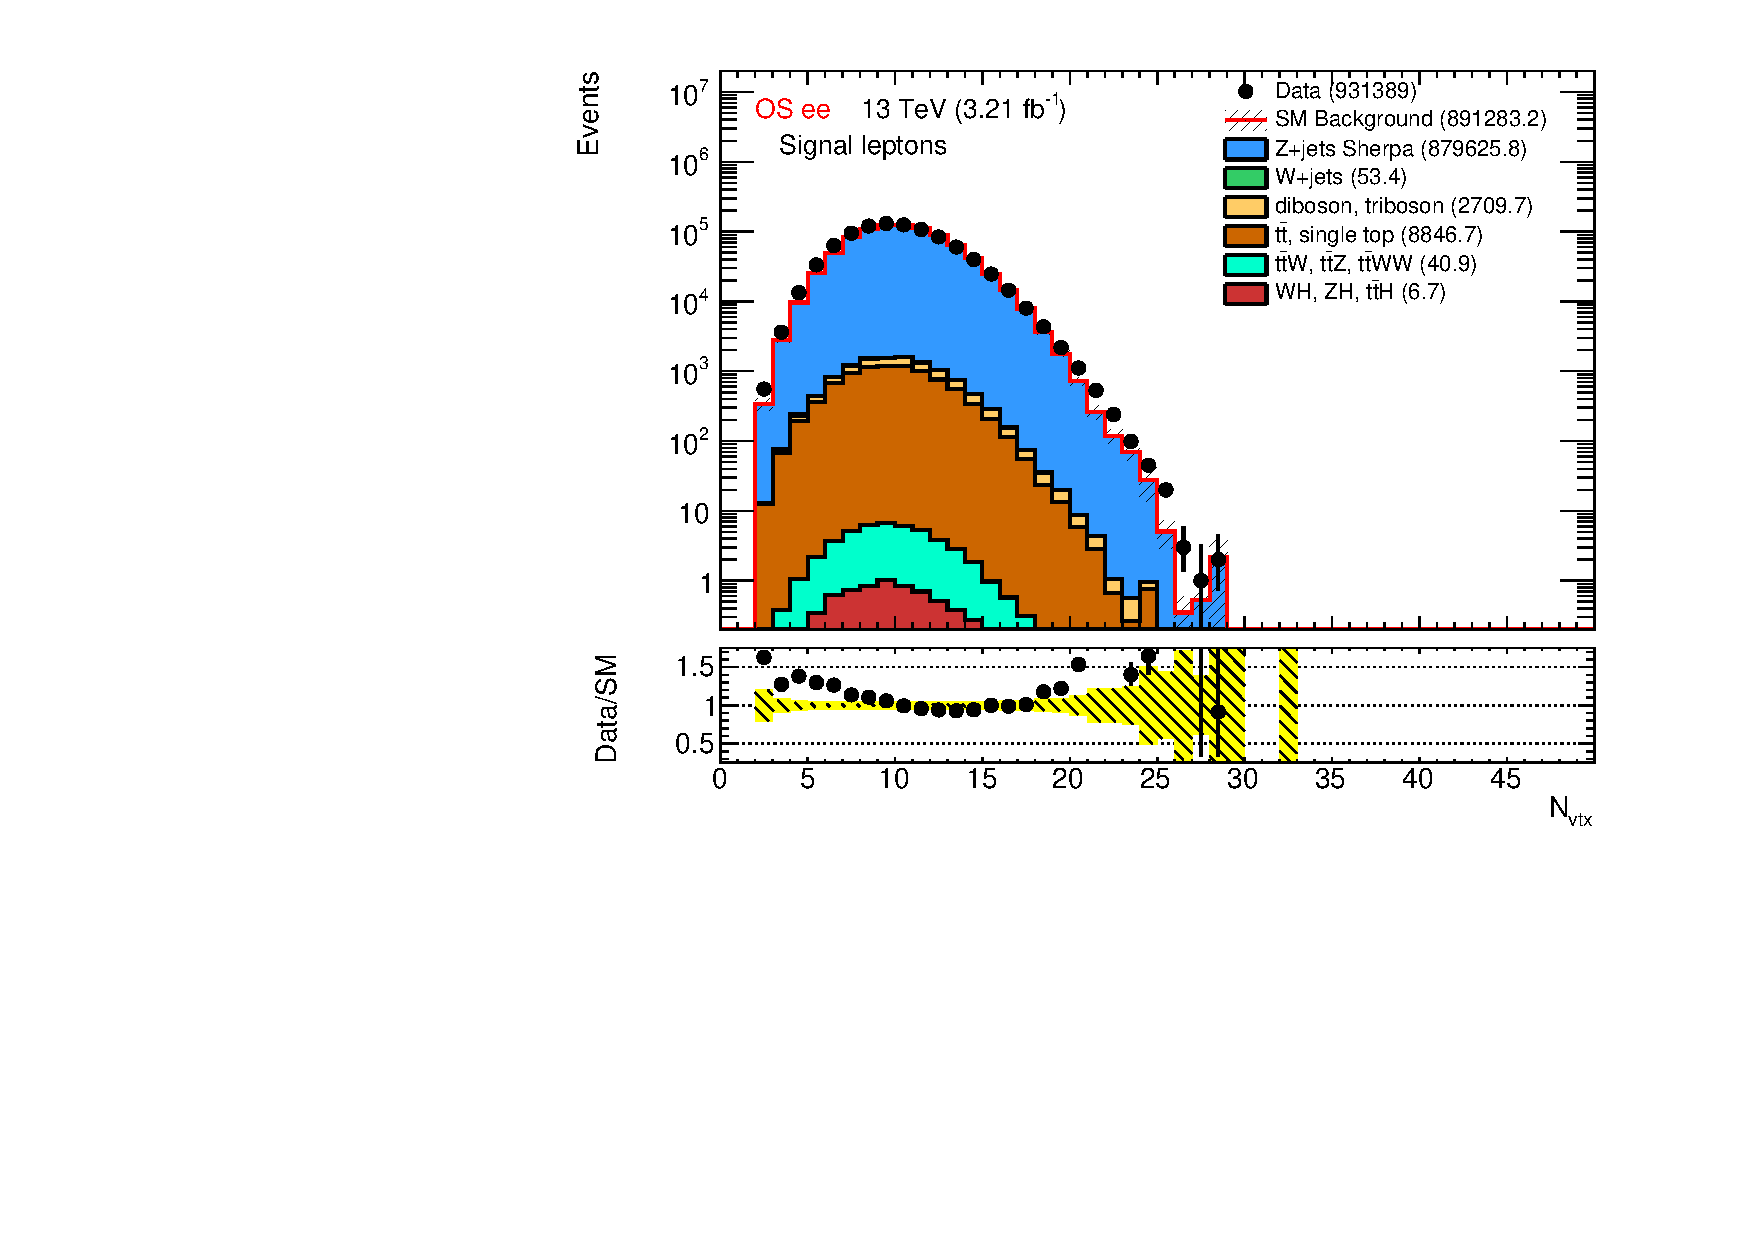
\includegraphics[width=0.45\textwidth]{DATAMC/NVTX_afterlepton_OSee_0_physics.pdf}}
{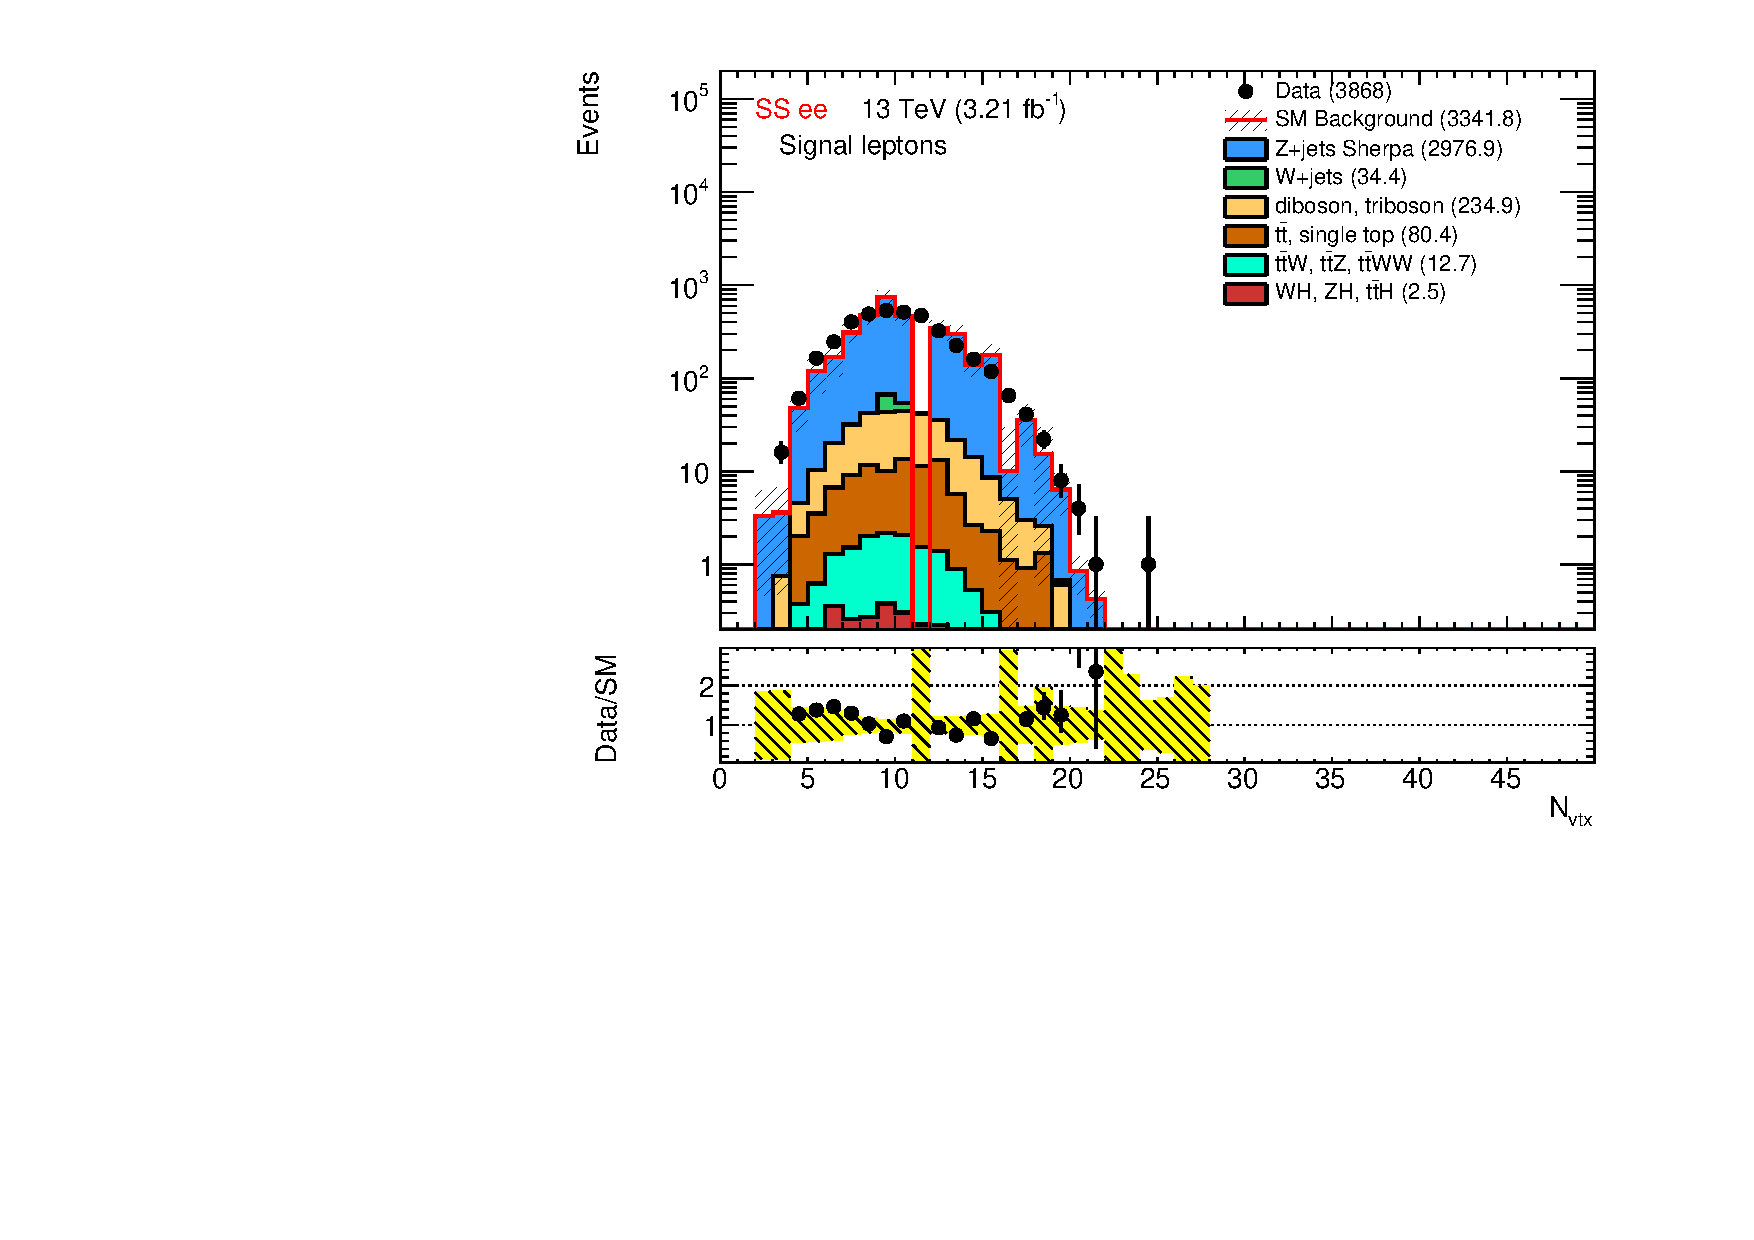
\includegraphics[width=0.45\textwidth]{DATAMC/NVTX_afterlepton_SSee_0_physics.pdf}}
{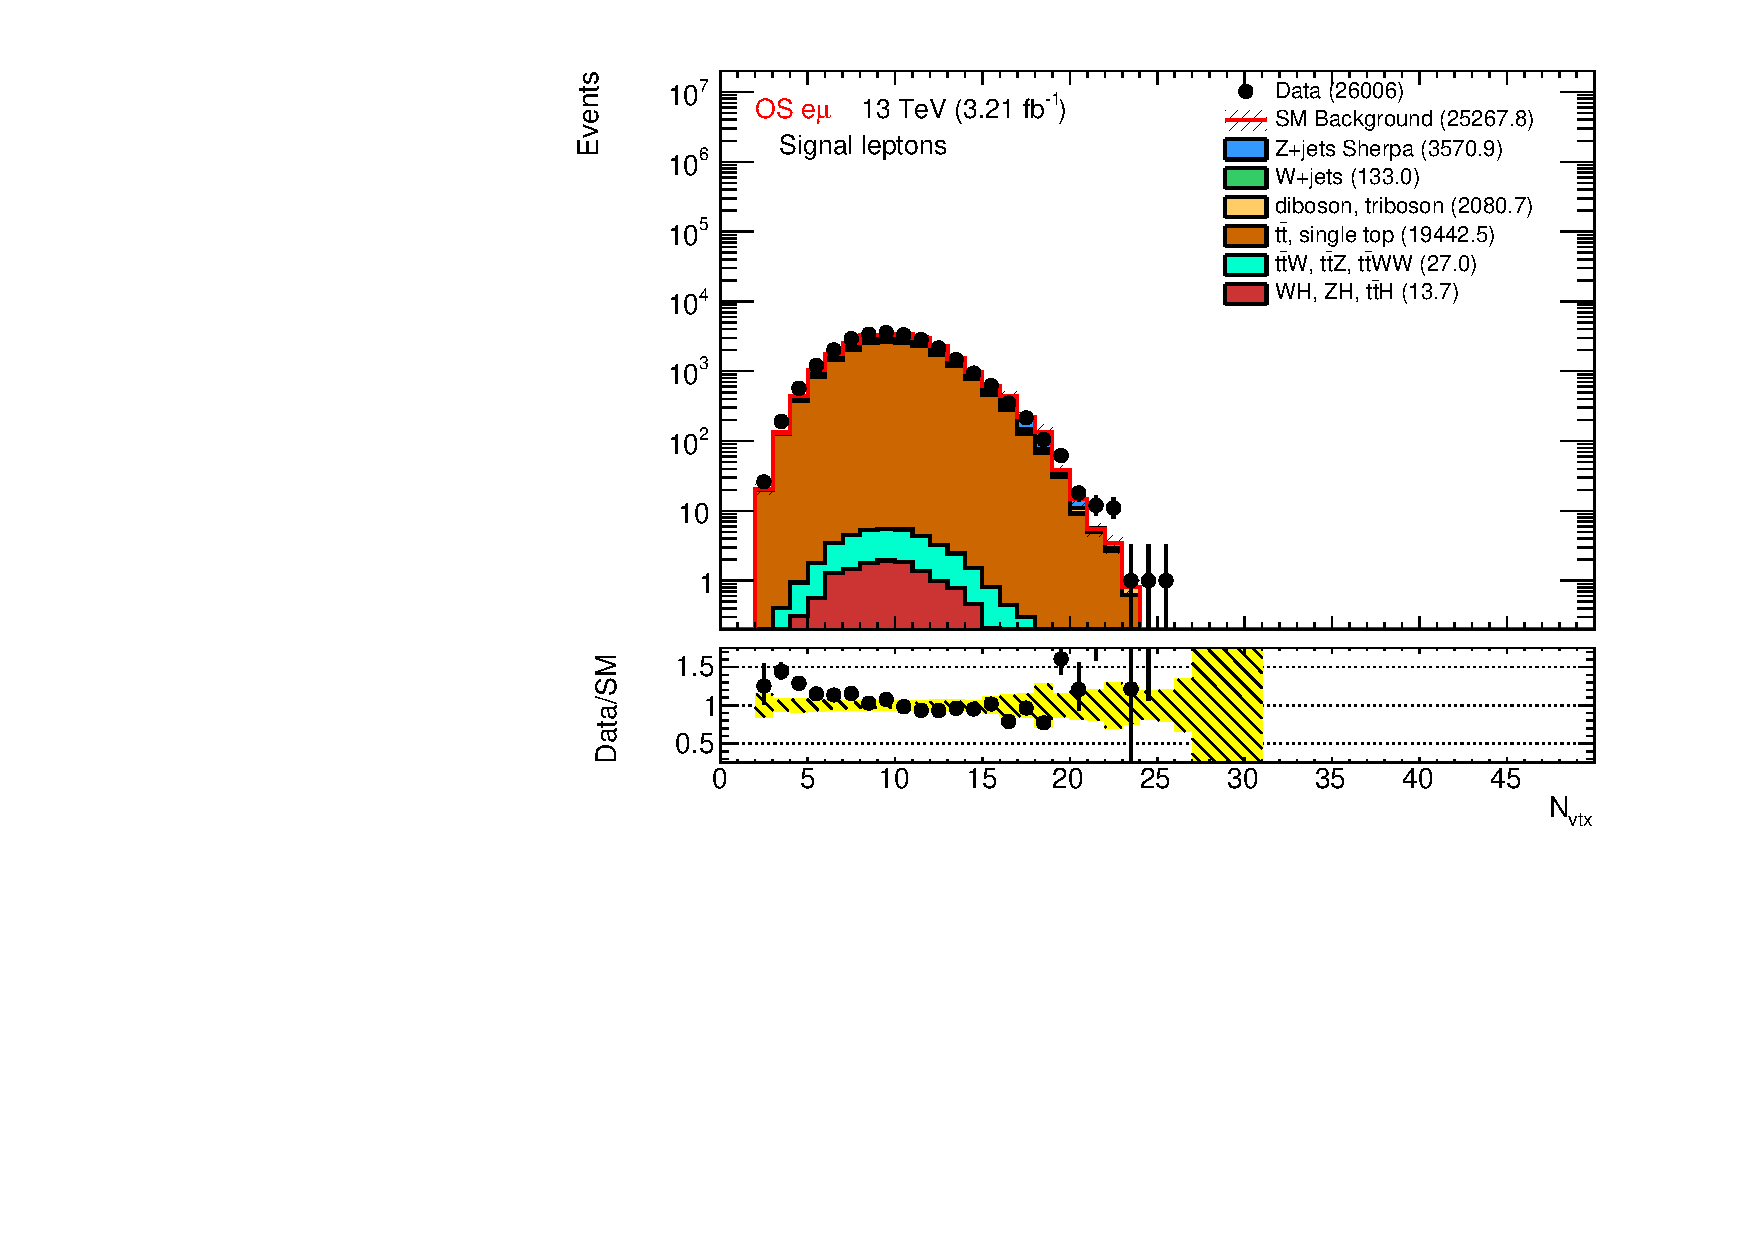
\includegraphics[width=0.45\textwidth]{DATAMC/NVTX_afterlepton_OSem_0_physics.pdf}}
{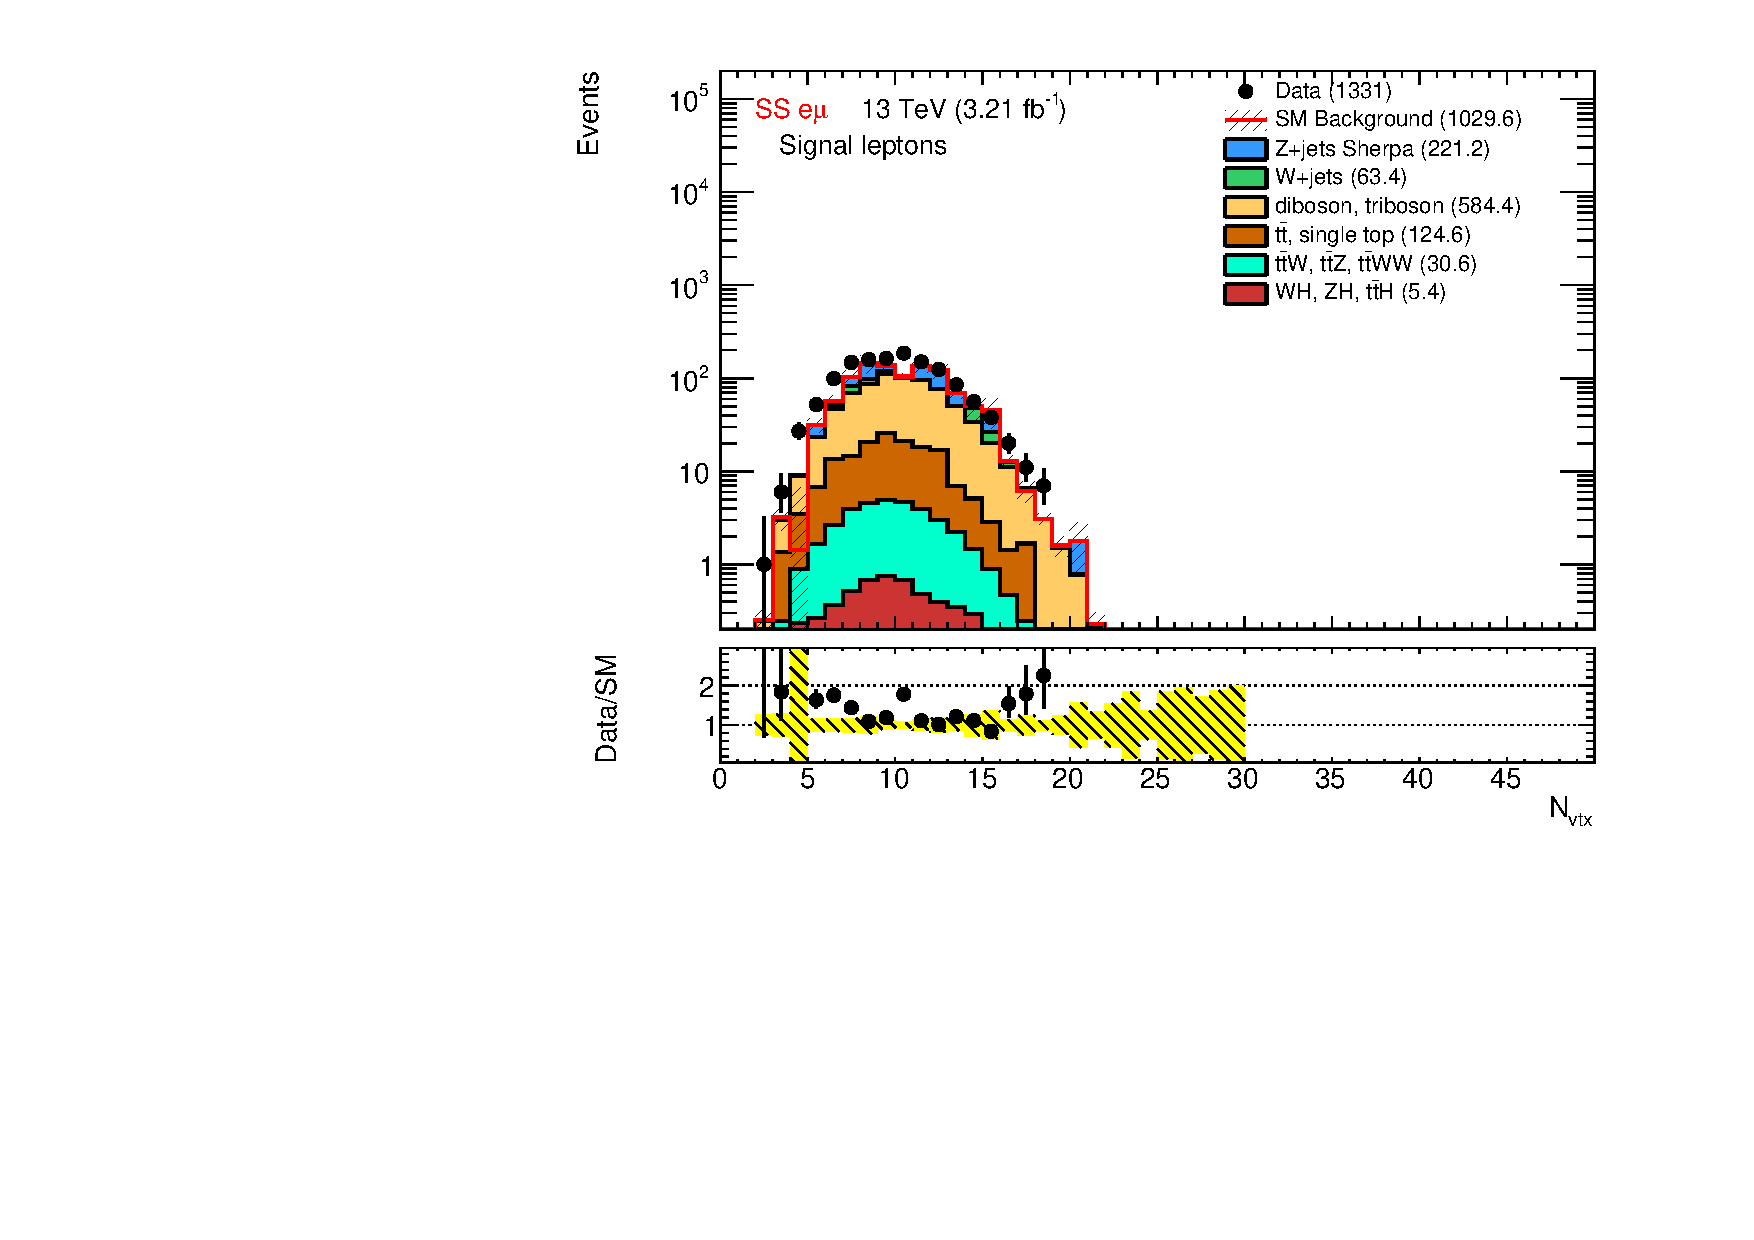
\includegraphics[width=0.45\textwidth]{DATAMC/NVTX_afterlepton_SSem_0_physics.pdf}}
{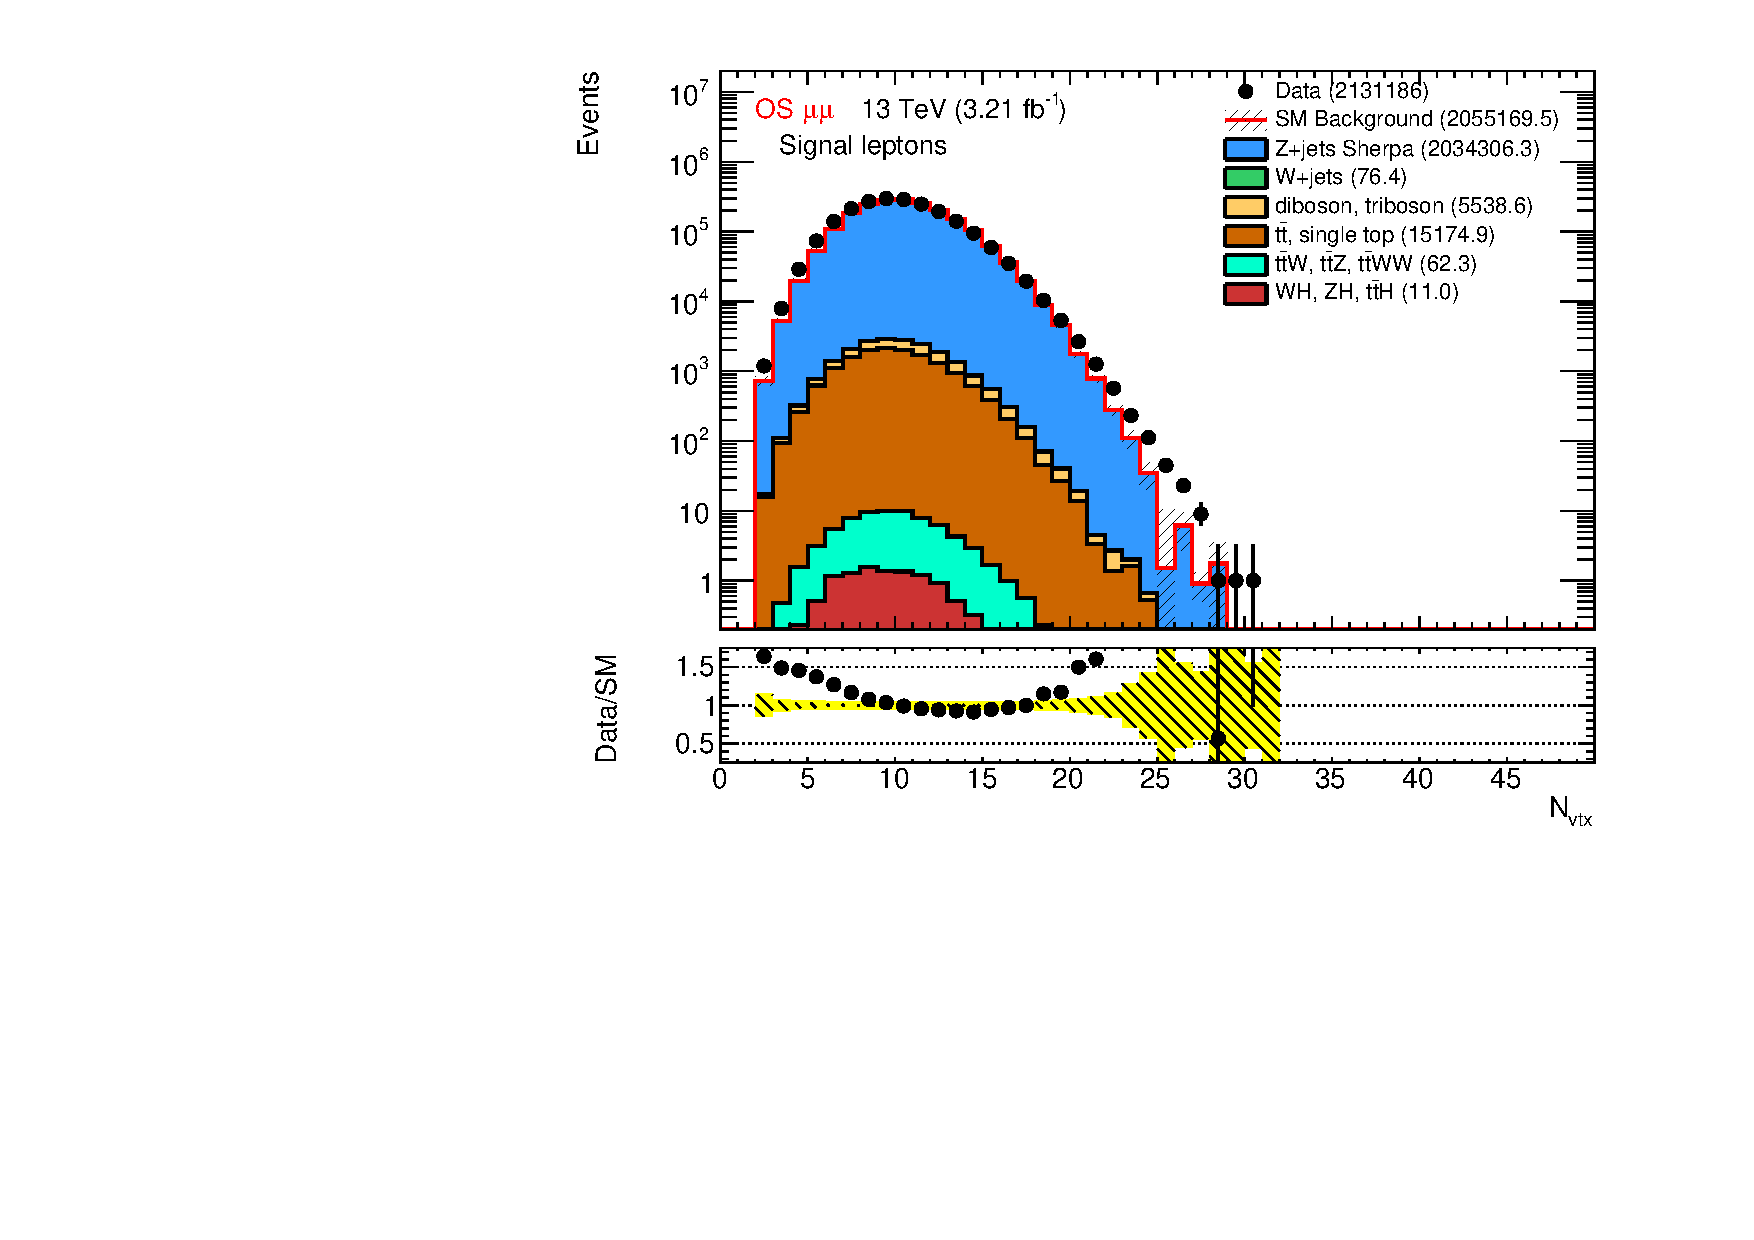
\includegraphics[width=0.45\textwidth]{DATAMC/NVTX_afterlepton_OSmm_0_physics.pdf}}
{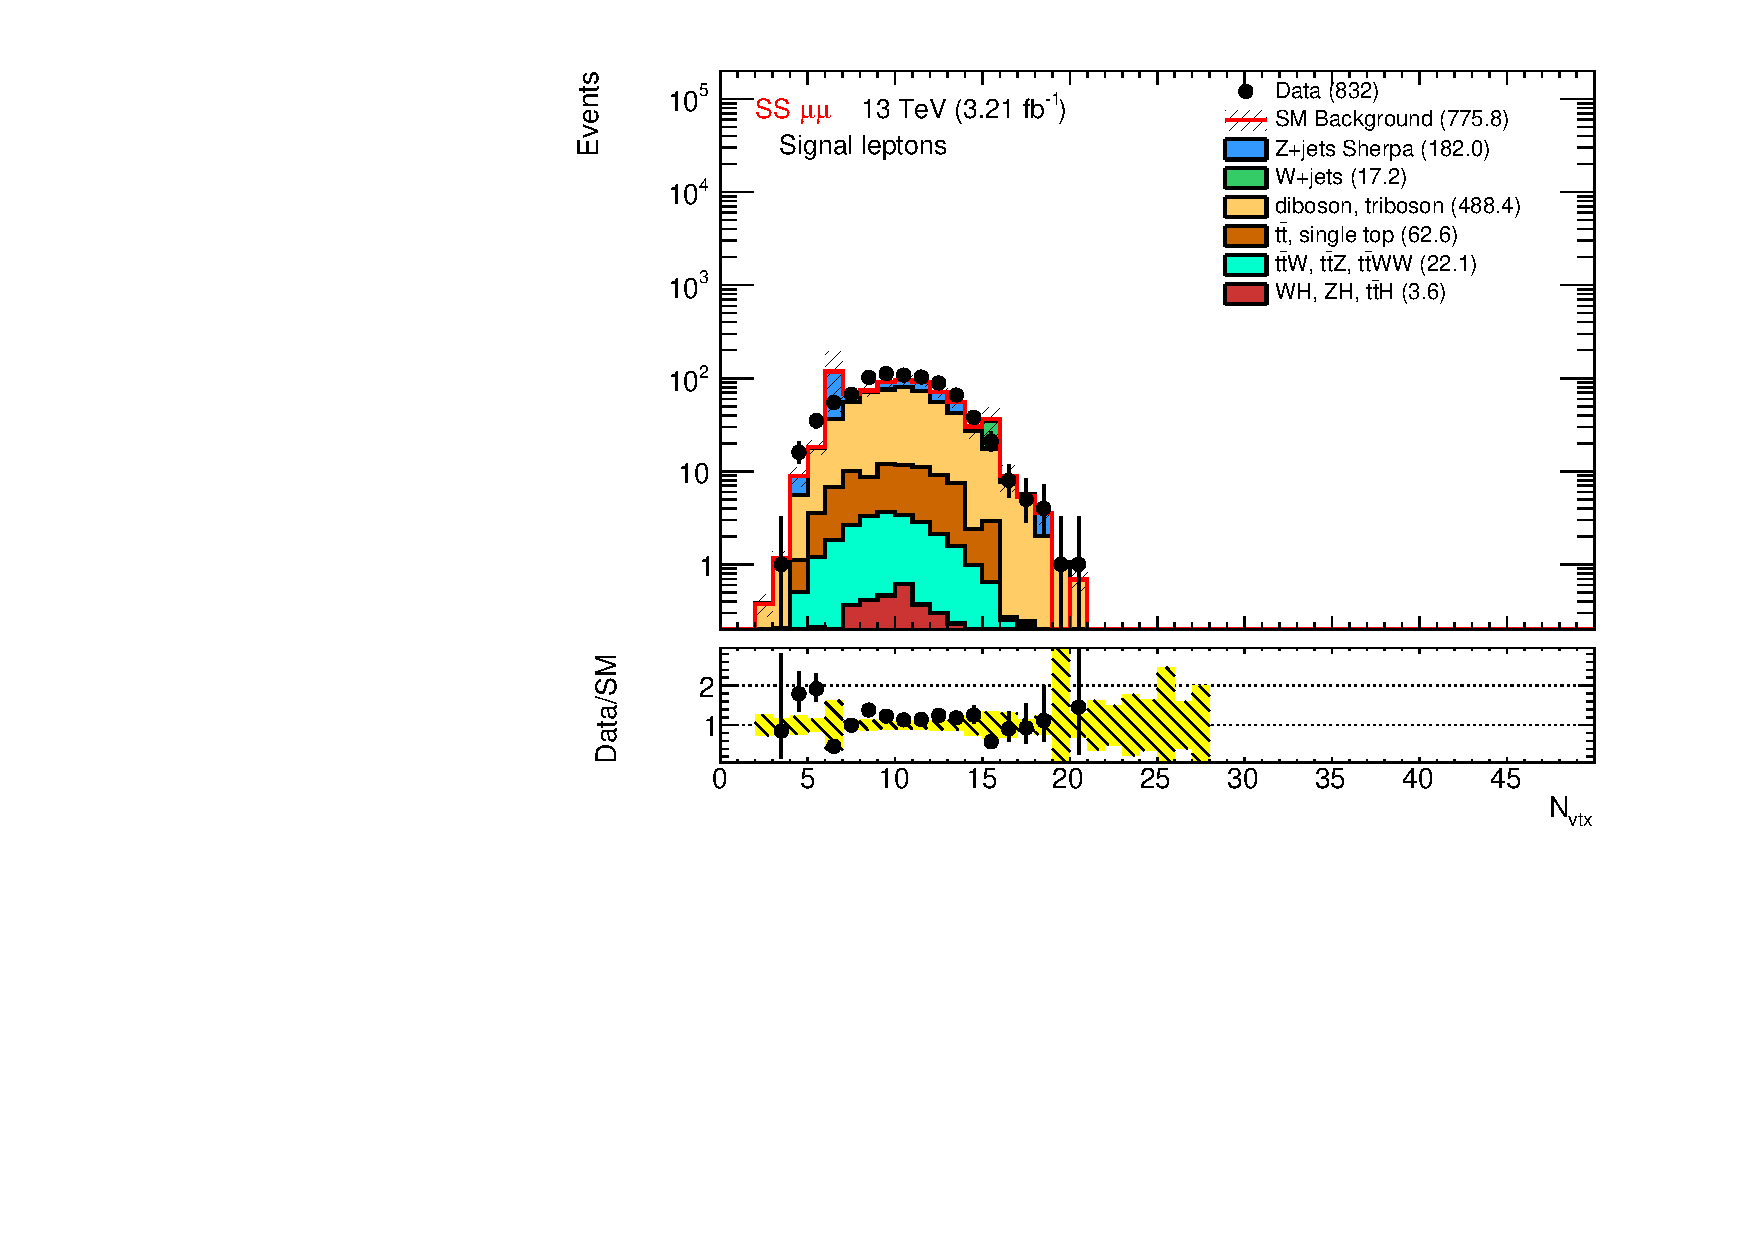
\includegraphics[width=0.45\textwidth]{DATAMC/NVTX_afterlepton_SSmm_0_physics.pdf}}
\caption{Distributions of the number of vertices for OS (left) and SS (right) in the $ee$ (top), $e\mu$ (middle) and $\mu\mu$ (bottom). The background contribution is taken directly from MC with no data-driven estimation of the background with fake and non-prompt leptons or charge mis-identification. Only luminosity and MC statistical uncertainties are included. Sherpa is used to model the $Z$+jets background.
}
\label{fig:app_Nvtx}
\end{figure}

\begin{figure}[htb!]
\centering
{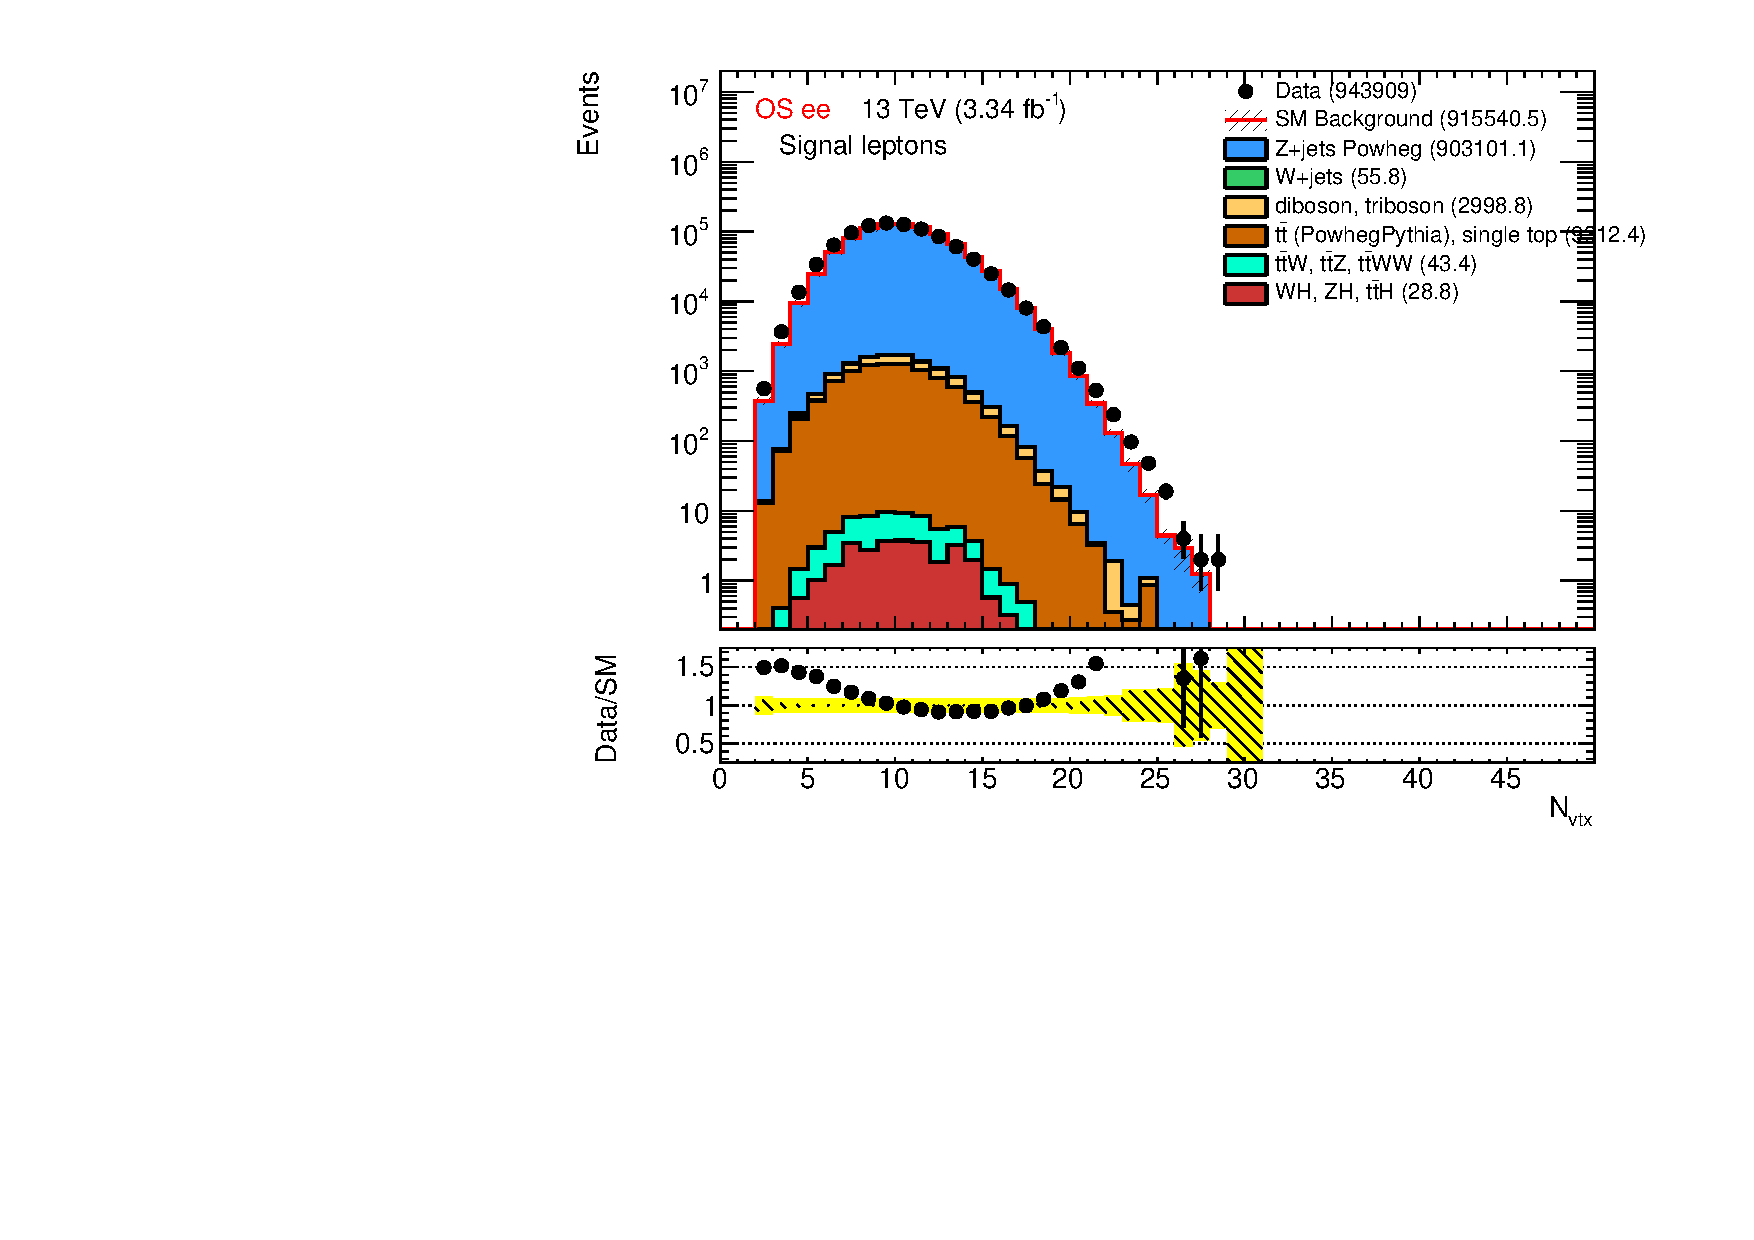
\includegraphics[width=0.45\textwidth]{DATAMC/NVTX_afterlepton_OSee_0_physics_powheg.pdf}}
{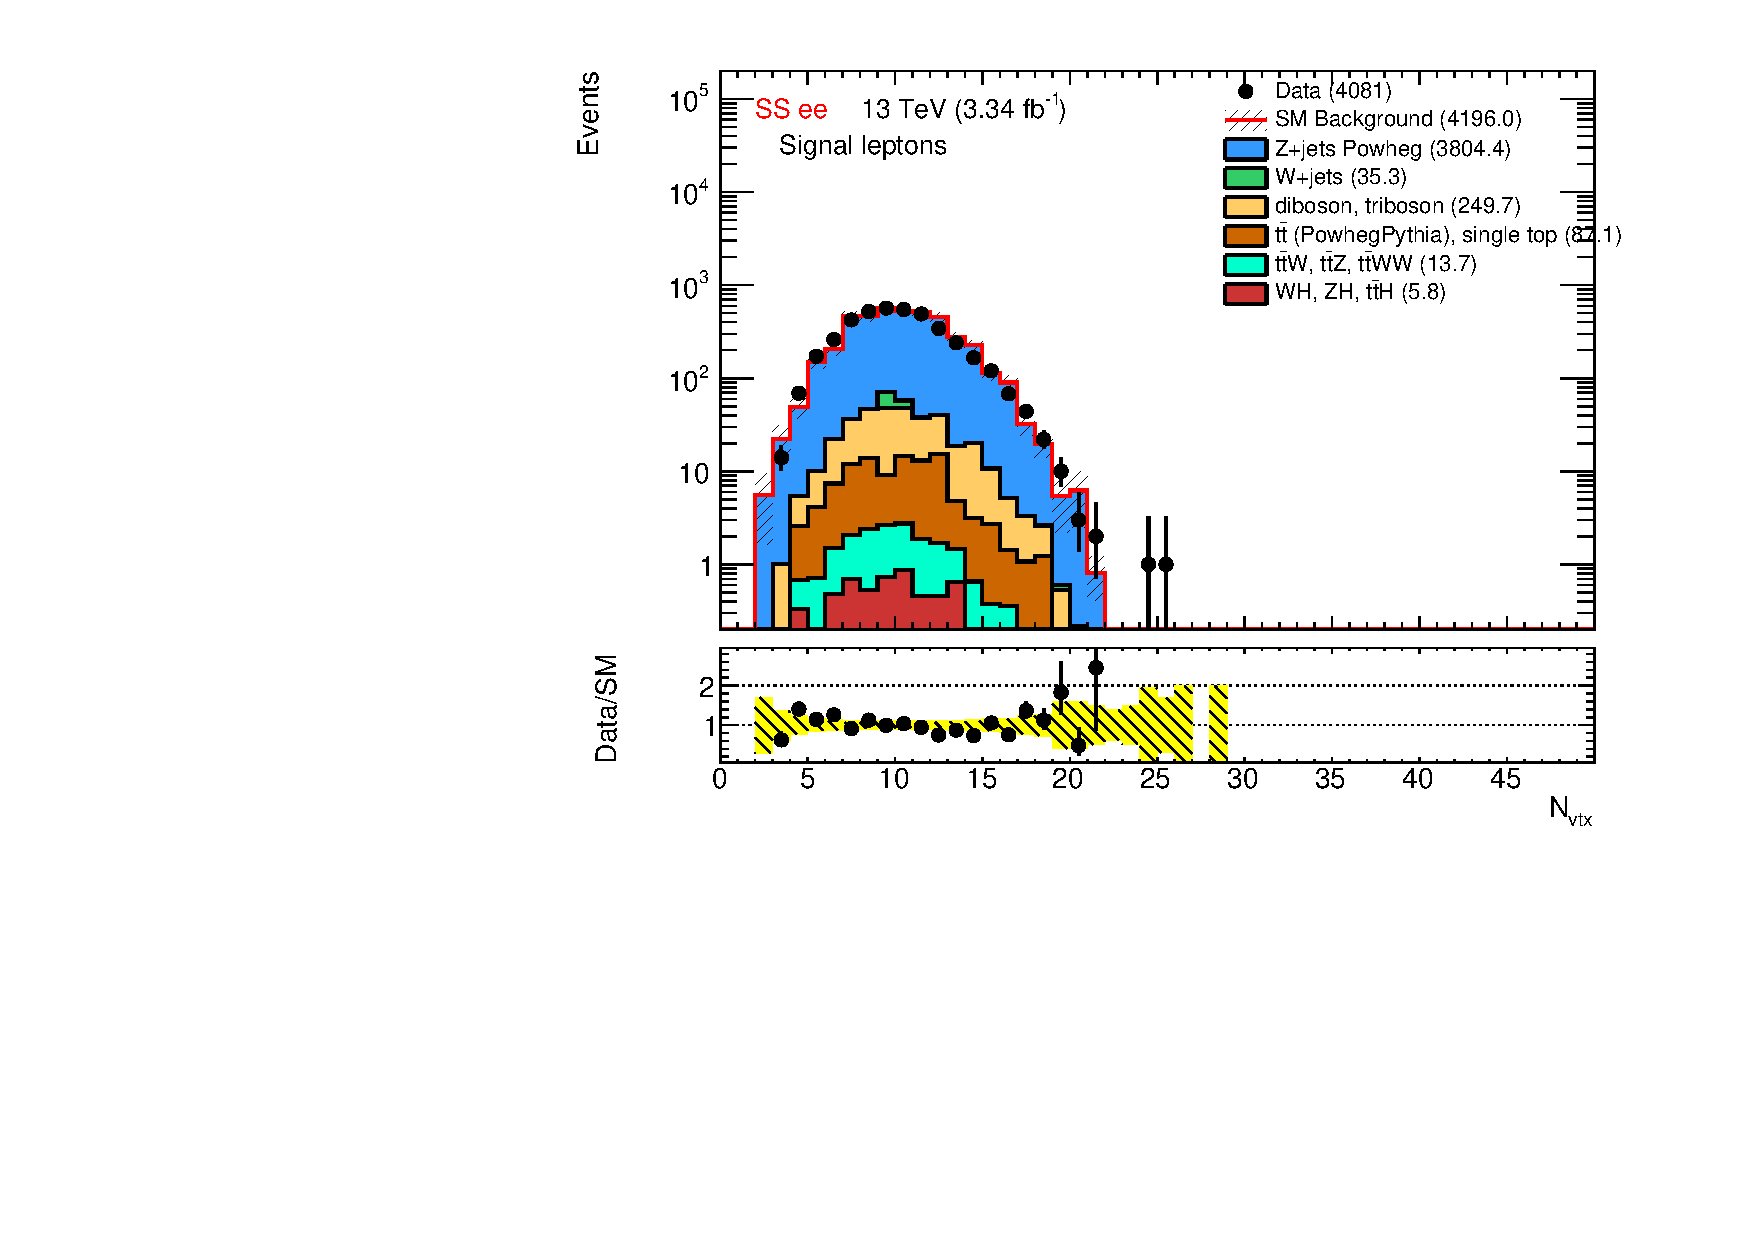
\includegraphics[width=0.45\textwidth]{DATAMC/NVTX_afterlepton_SSee_0_physics_powheg.pdf}}
{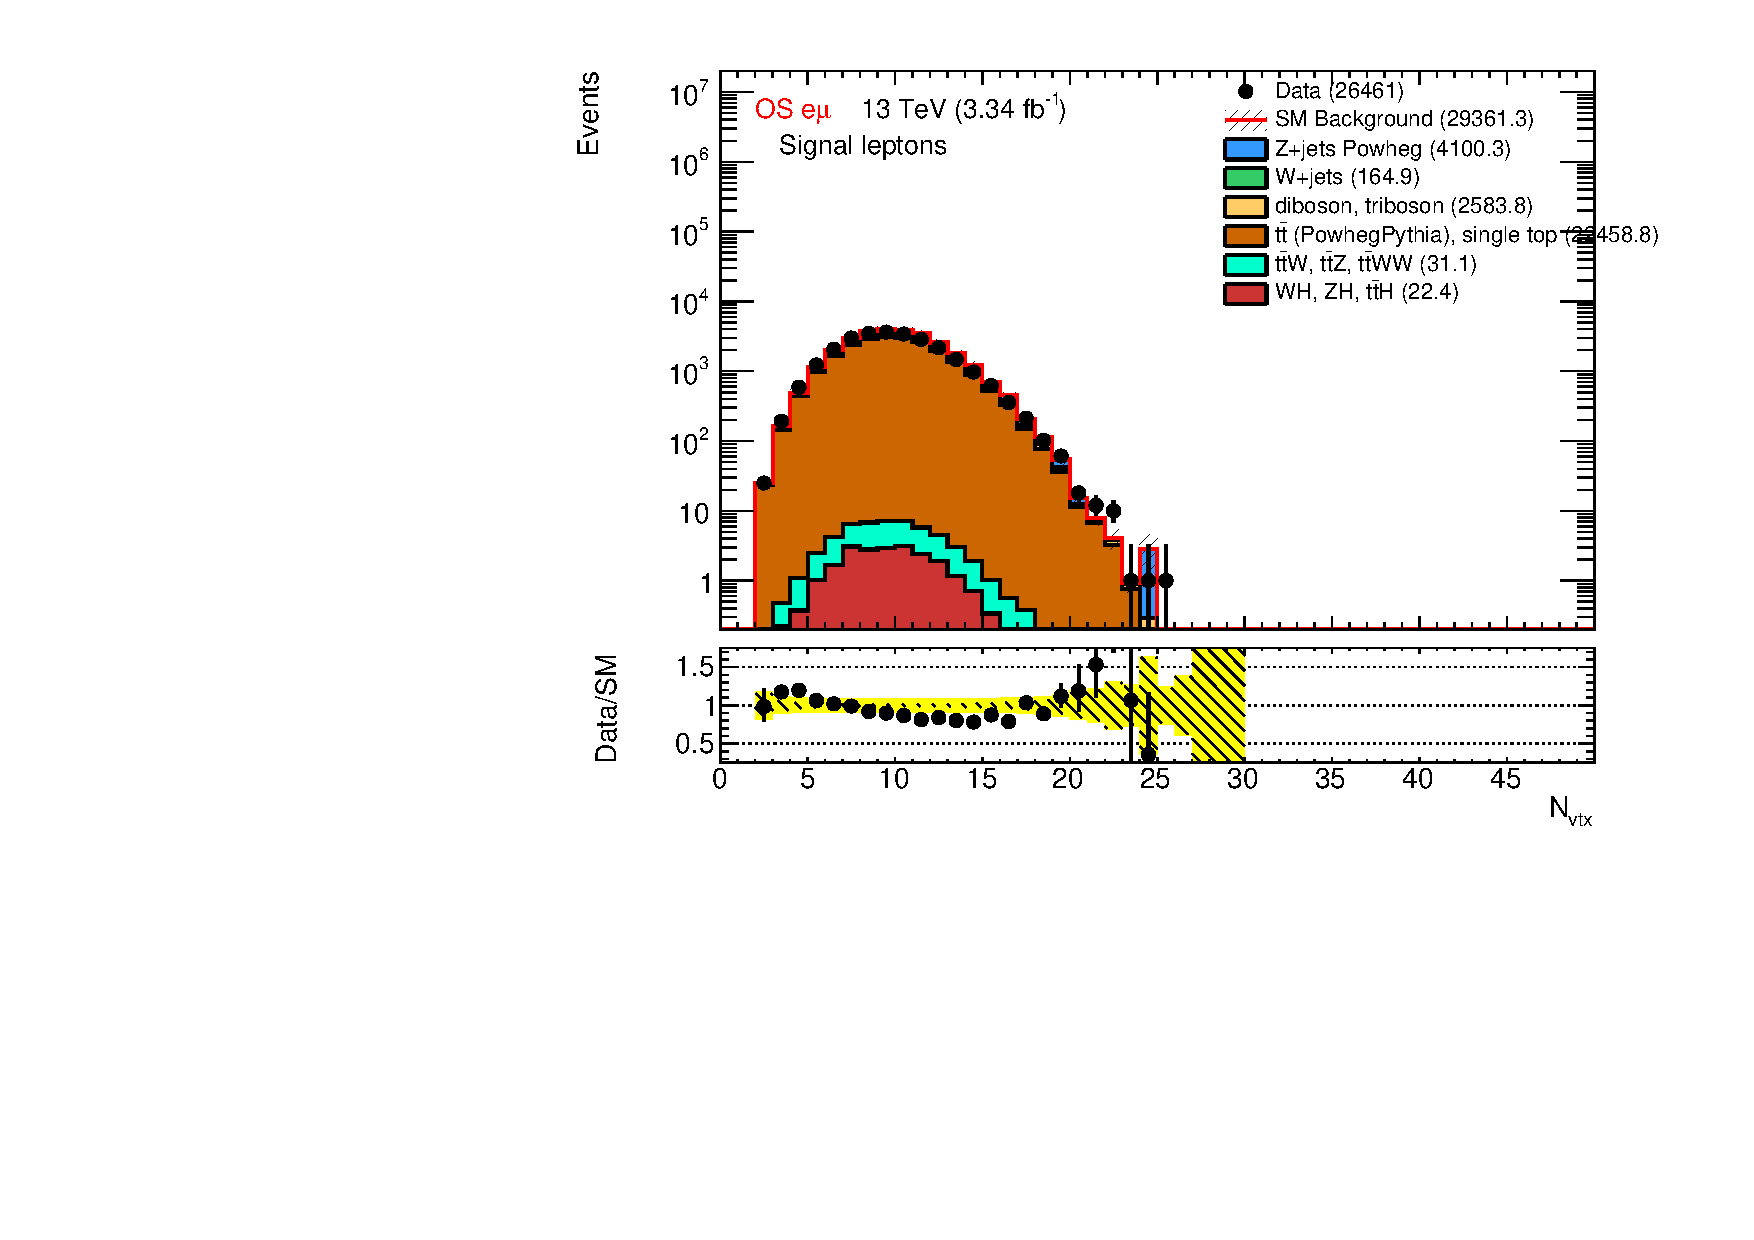
\includegraphics[width=0.45\textwidth]{DATAMC/NVTX_afterlepton_OSem_0_physics_powheg.pdf}}
{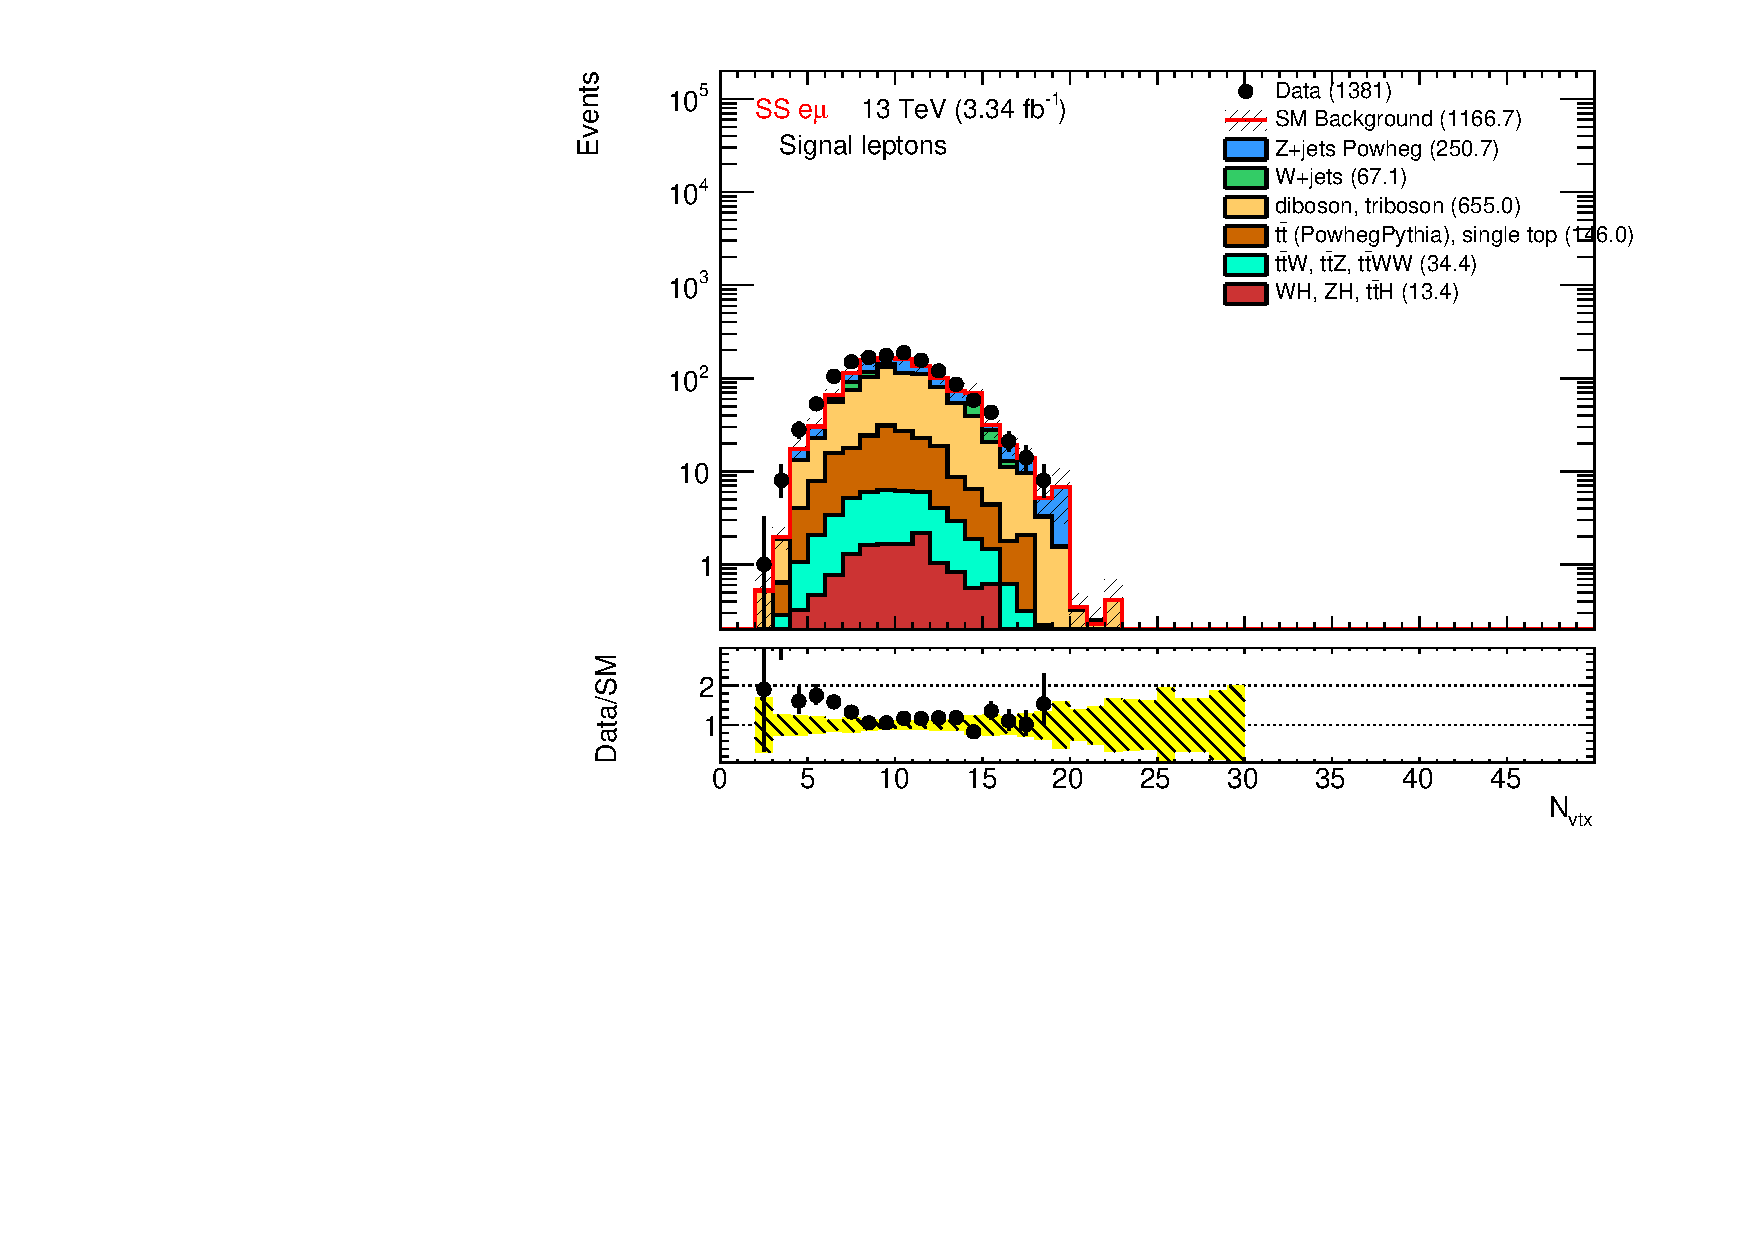
\includegraphics[width=0.45\textwidth]{DATAMC/NVTX_afterlepton_SSem_0_physics_powheg.pdf}}
{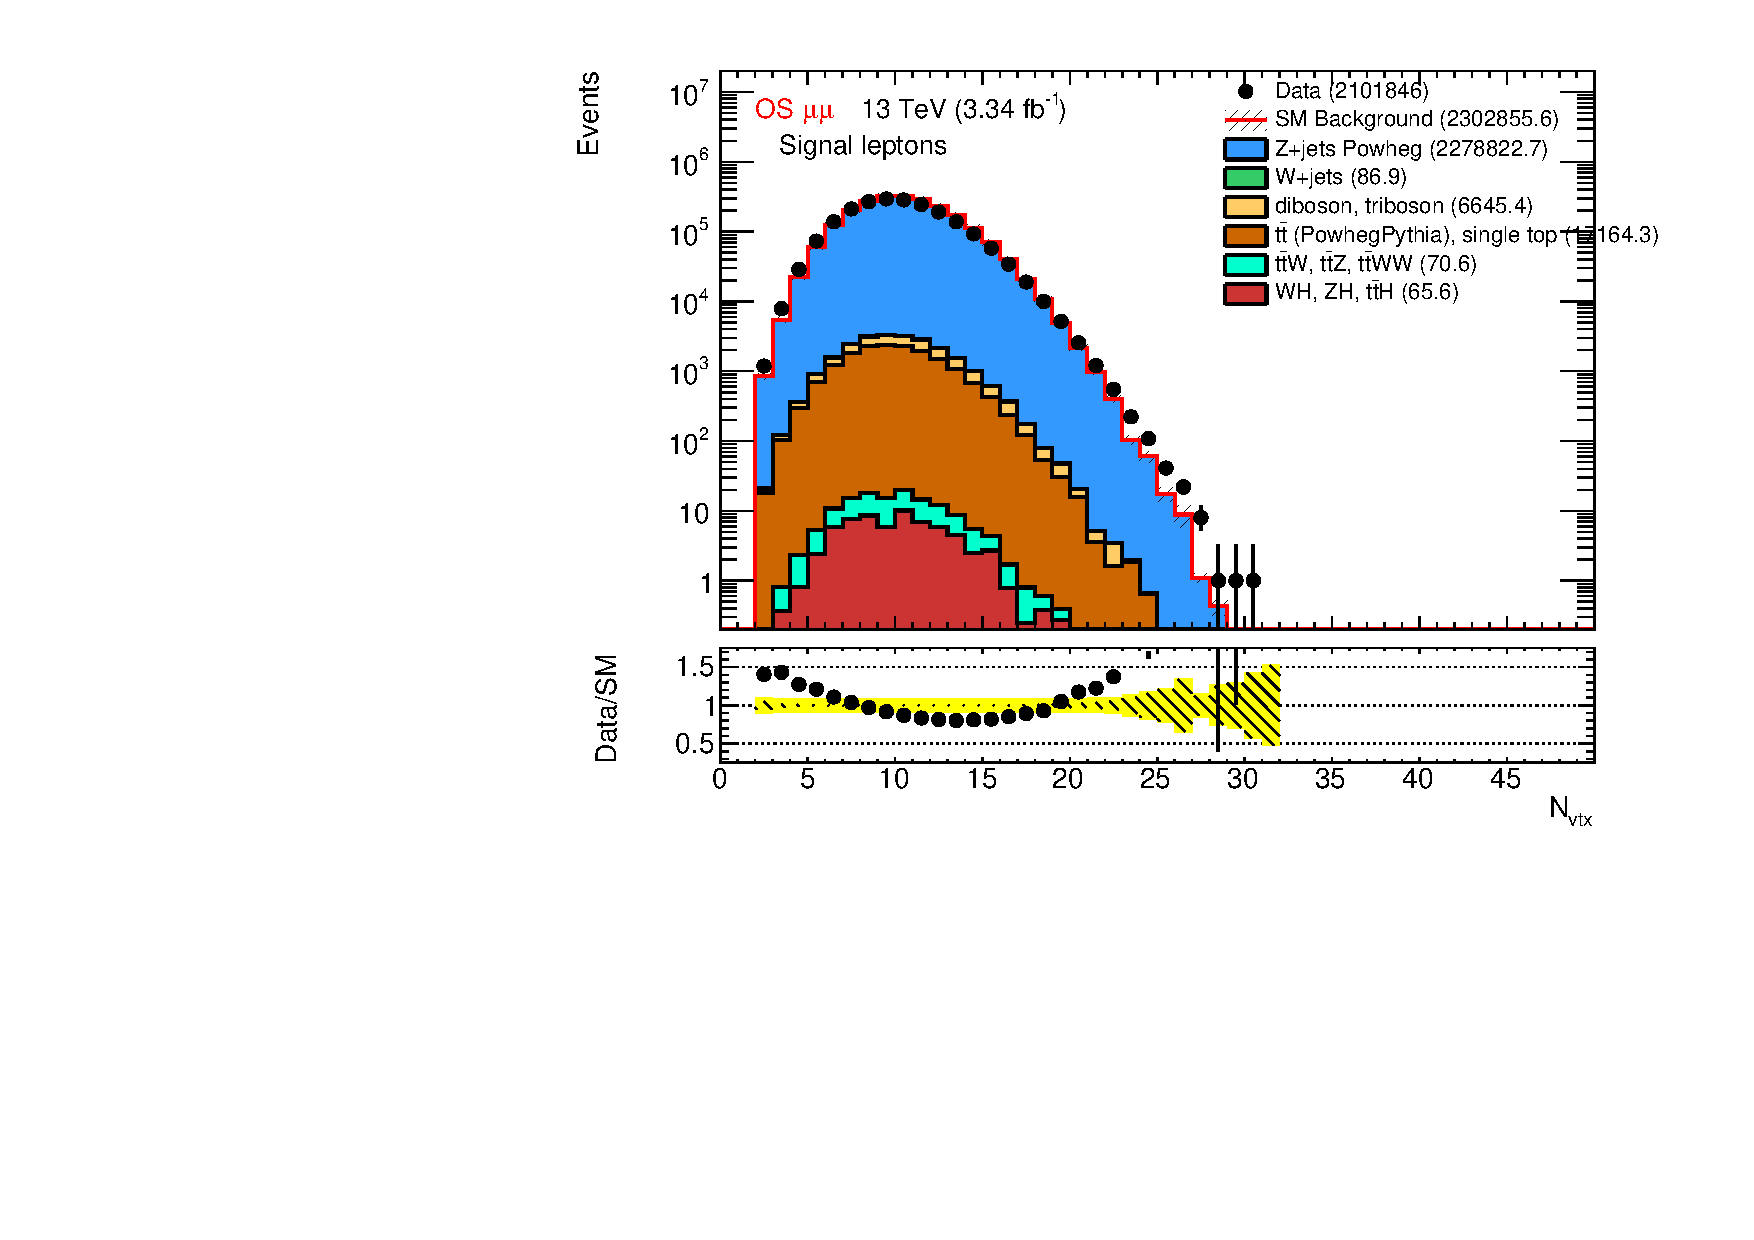
\includegraphics[width=0.45\textwidth]{DATAMC/NVTX_afterlepton_OSmm_0_physics_powheg.pdf}}
{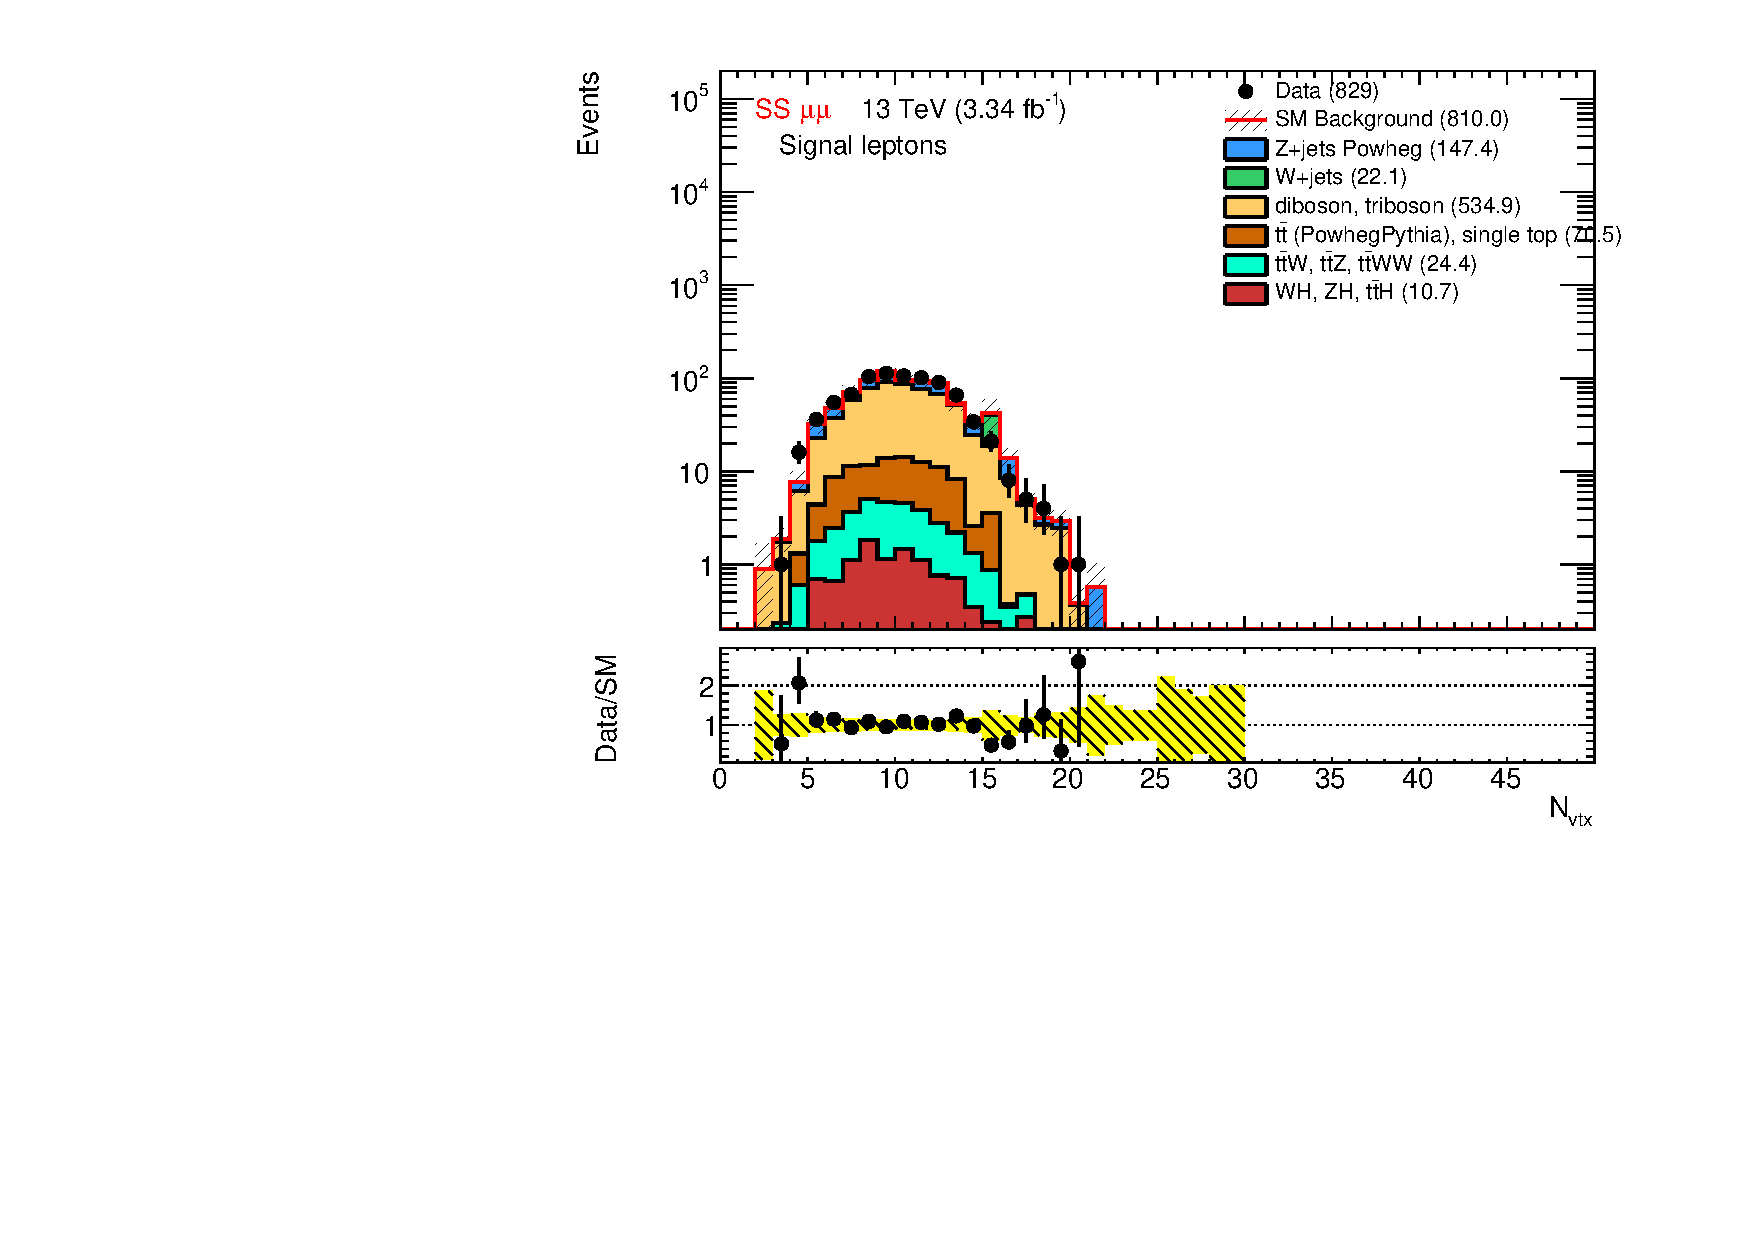
\includegraphics[width=0.45\textwidth]{DATAMC/NVTX_afterlepton_SSmm_0_physics_powheg.pdf}}
\caption{Distributions of the number of vertices for OS (left) and SS (right) in the $ee$ (top), $e\mu$ (middle) and $\mu\mu$ (bottom). The background contribution is taken directly from MC with no data-driven estimation of the background with fake and non-prompt leptons or charge mis-identification. Only luminosity and MC statistical uncertainties are included. Powheg is used to model the $Z$+jets background.
}
\label{fig:app_Nvtx_powheg}
\end{figure}

\begin{figure}[htb!]
\centering
{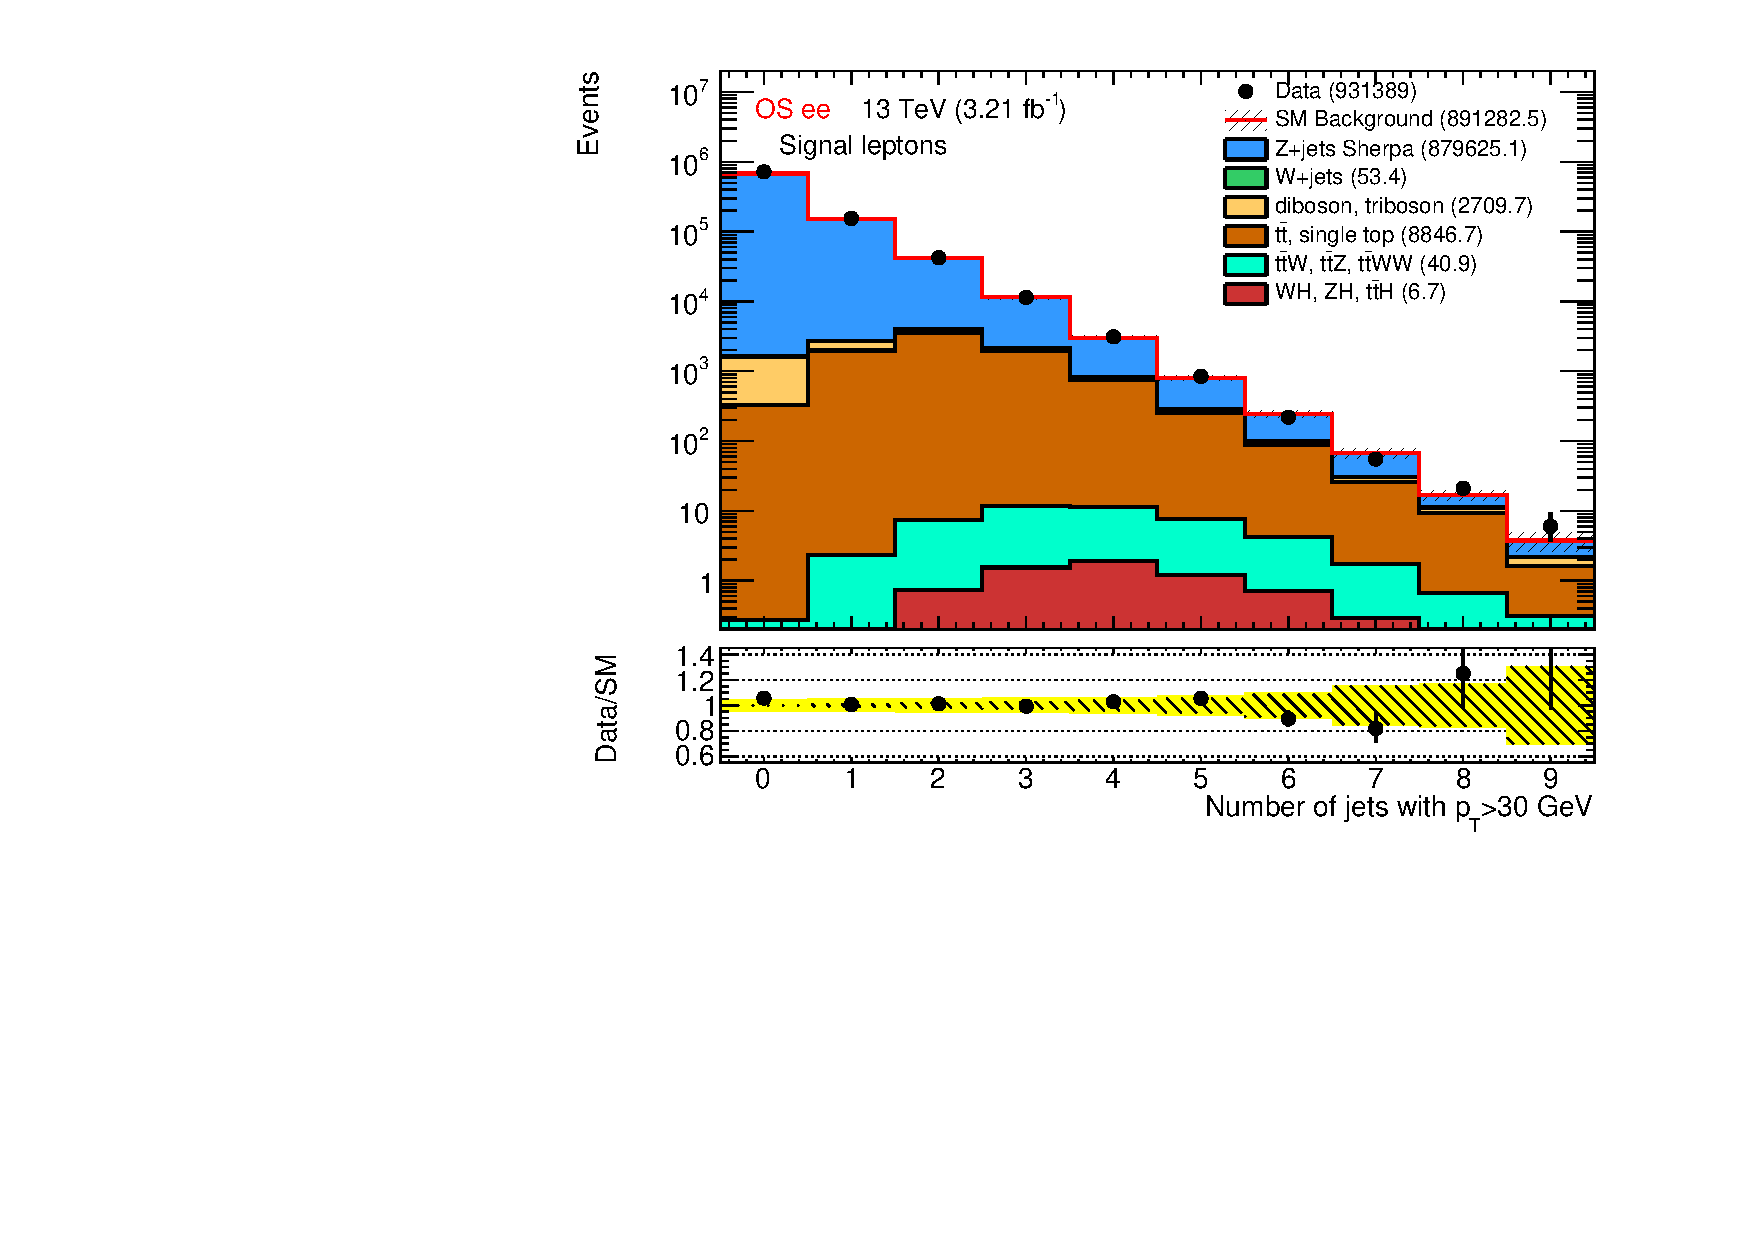
\includegraphics[width=0.45\textwidth]{DATAMC/NJET30_afterlepton_OSee_0_physics.pdf}}
{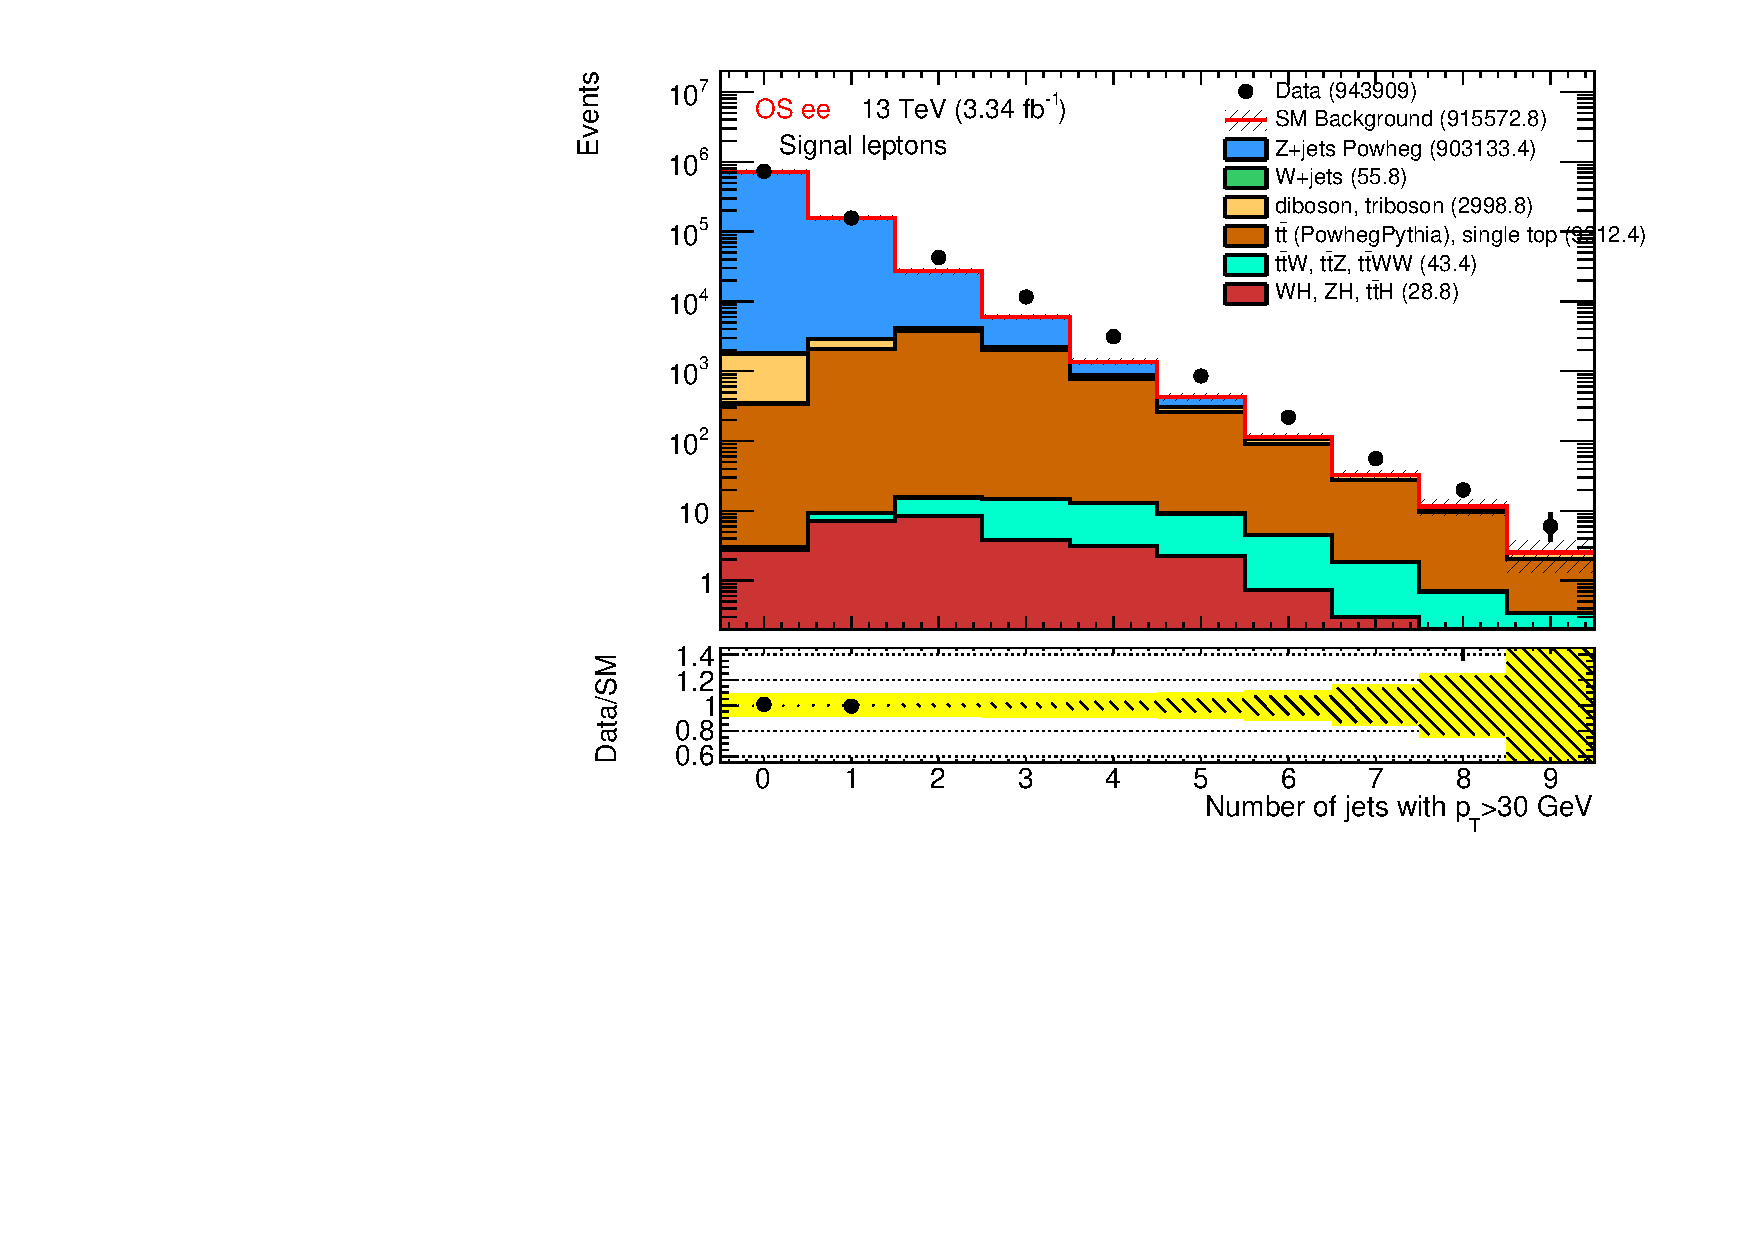
\includegraphics[width=0.45\textwidth]{DATAMC/NJET30_afterlepton_OSee_0_physics_powheg.pdf}}
{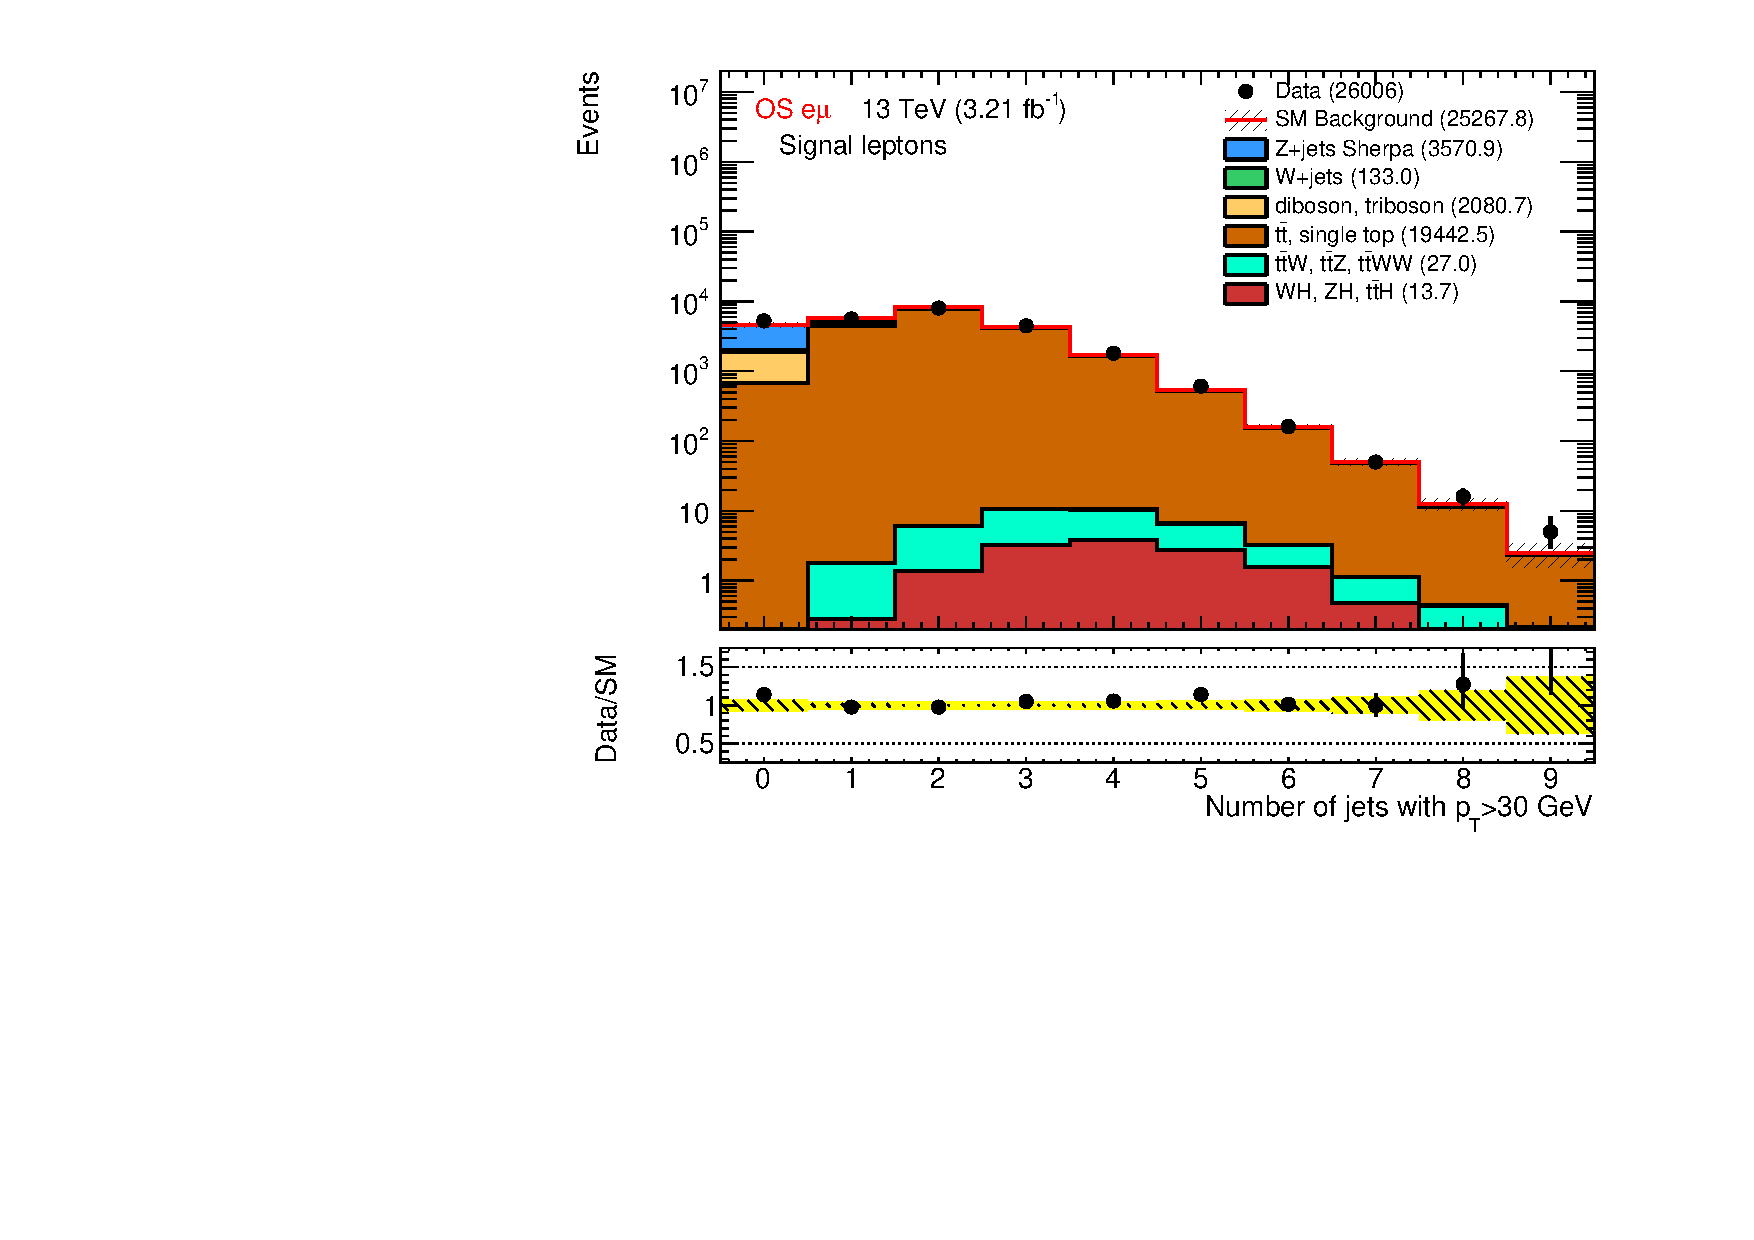
\includegraphics[width=0.45\textwidth]{DATAMC/NJET30_afterlepton_OSem_0_physics.pdf}}
{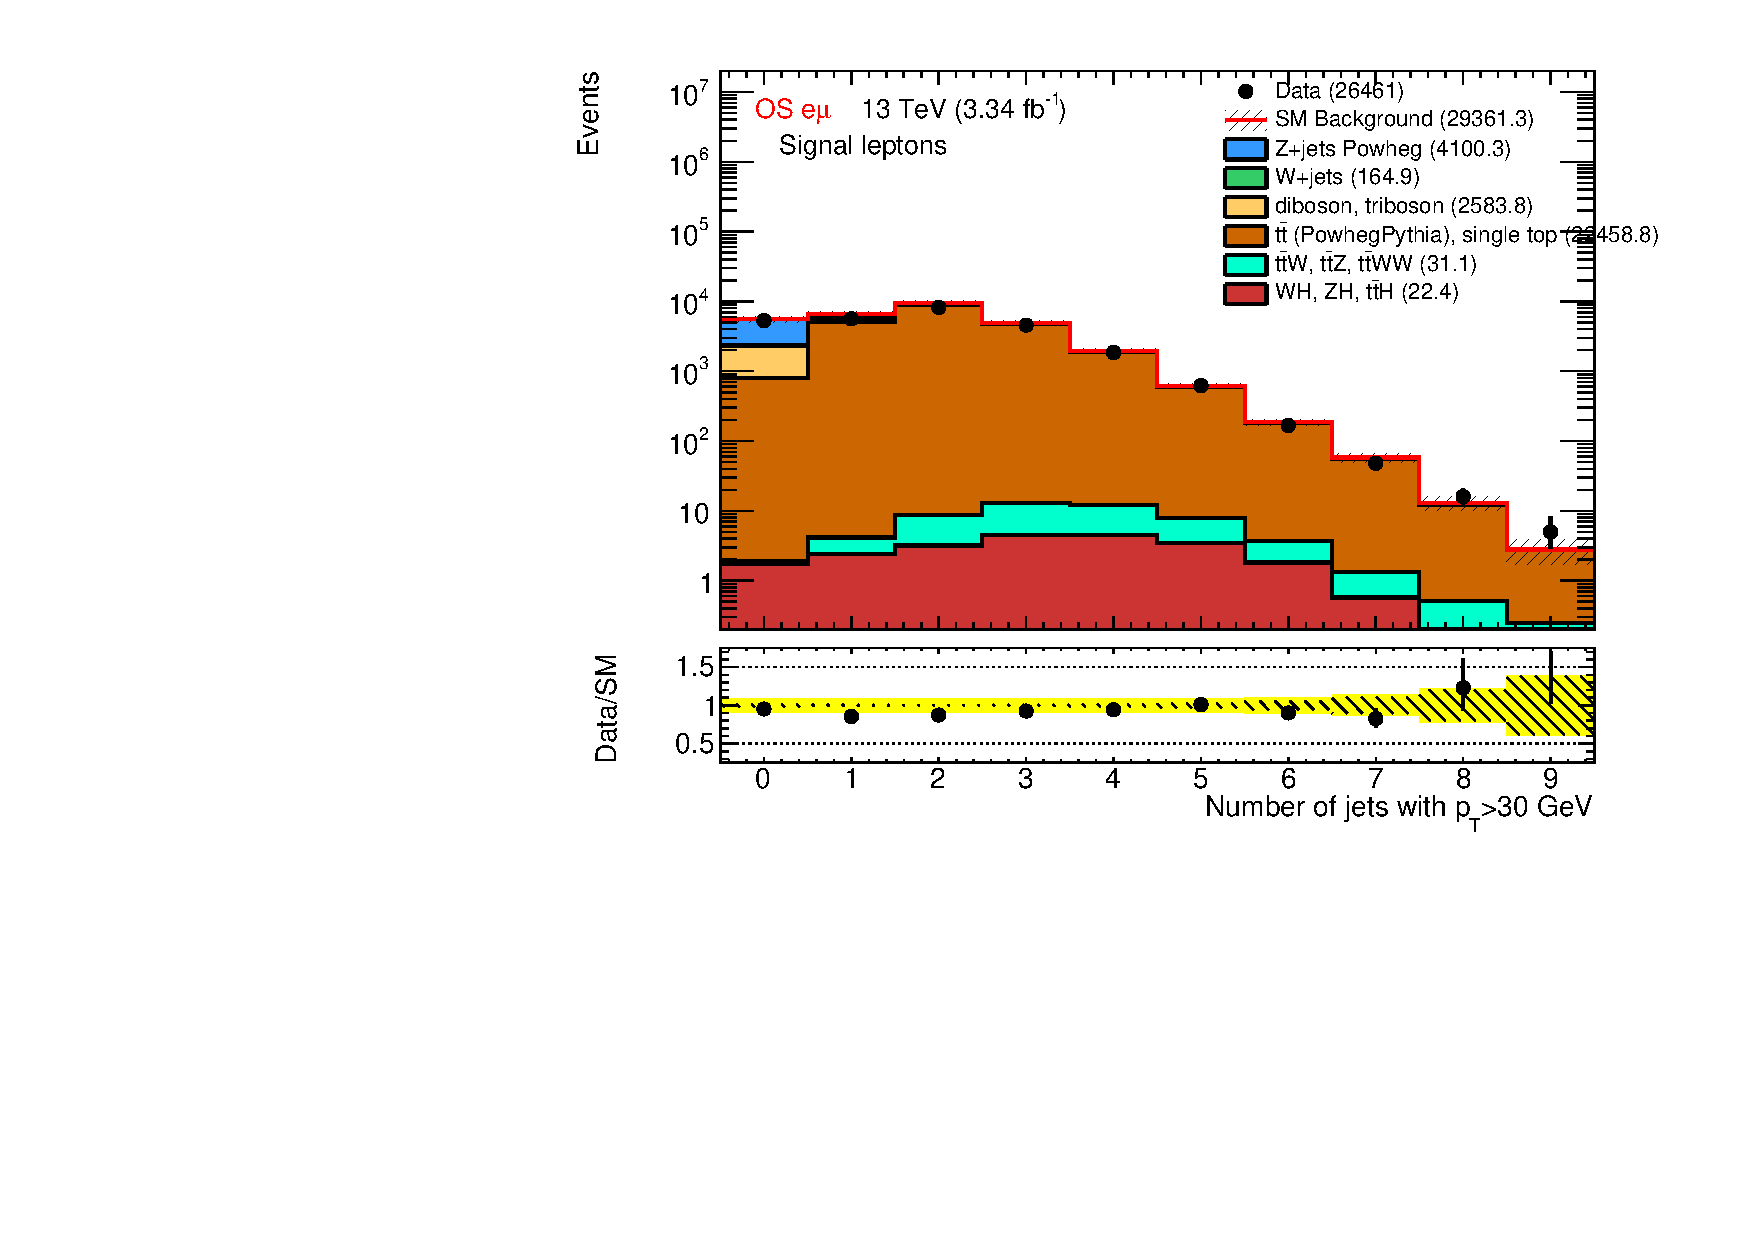
\includegraphics[width=0.45\textwidth]{DATAMC/NJET30_afterlepton_OSem_0_physics_powheg.pdf}}
{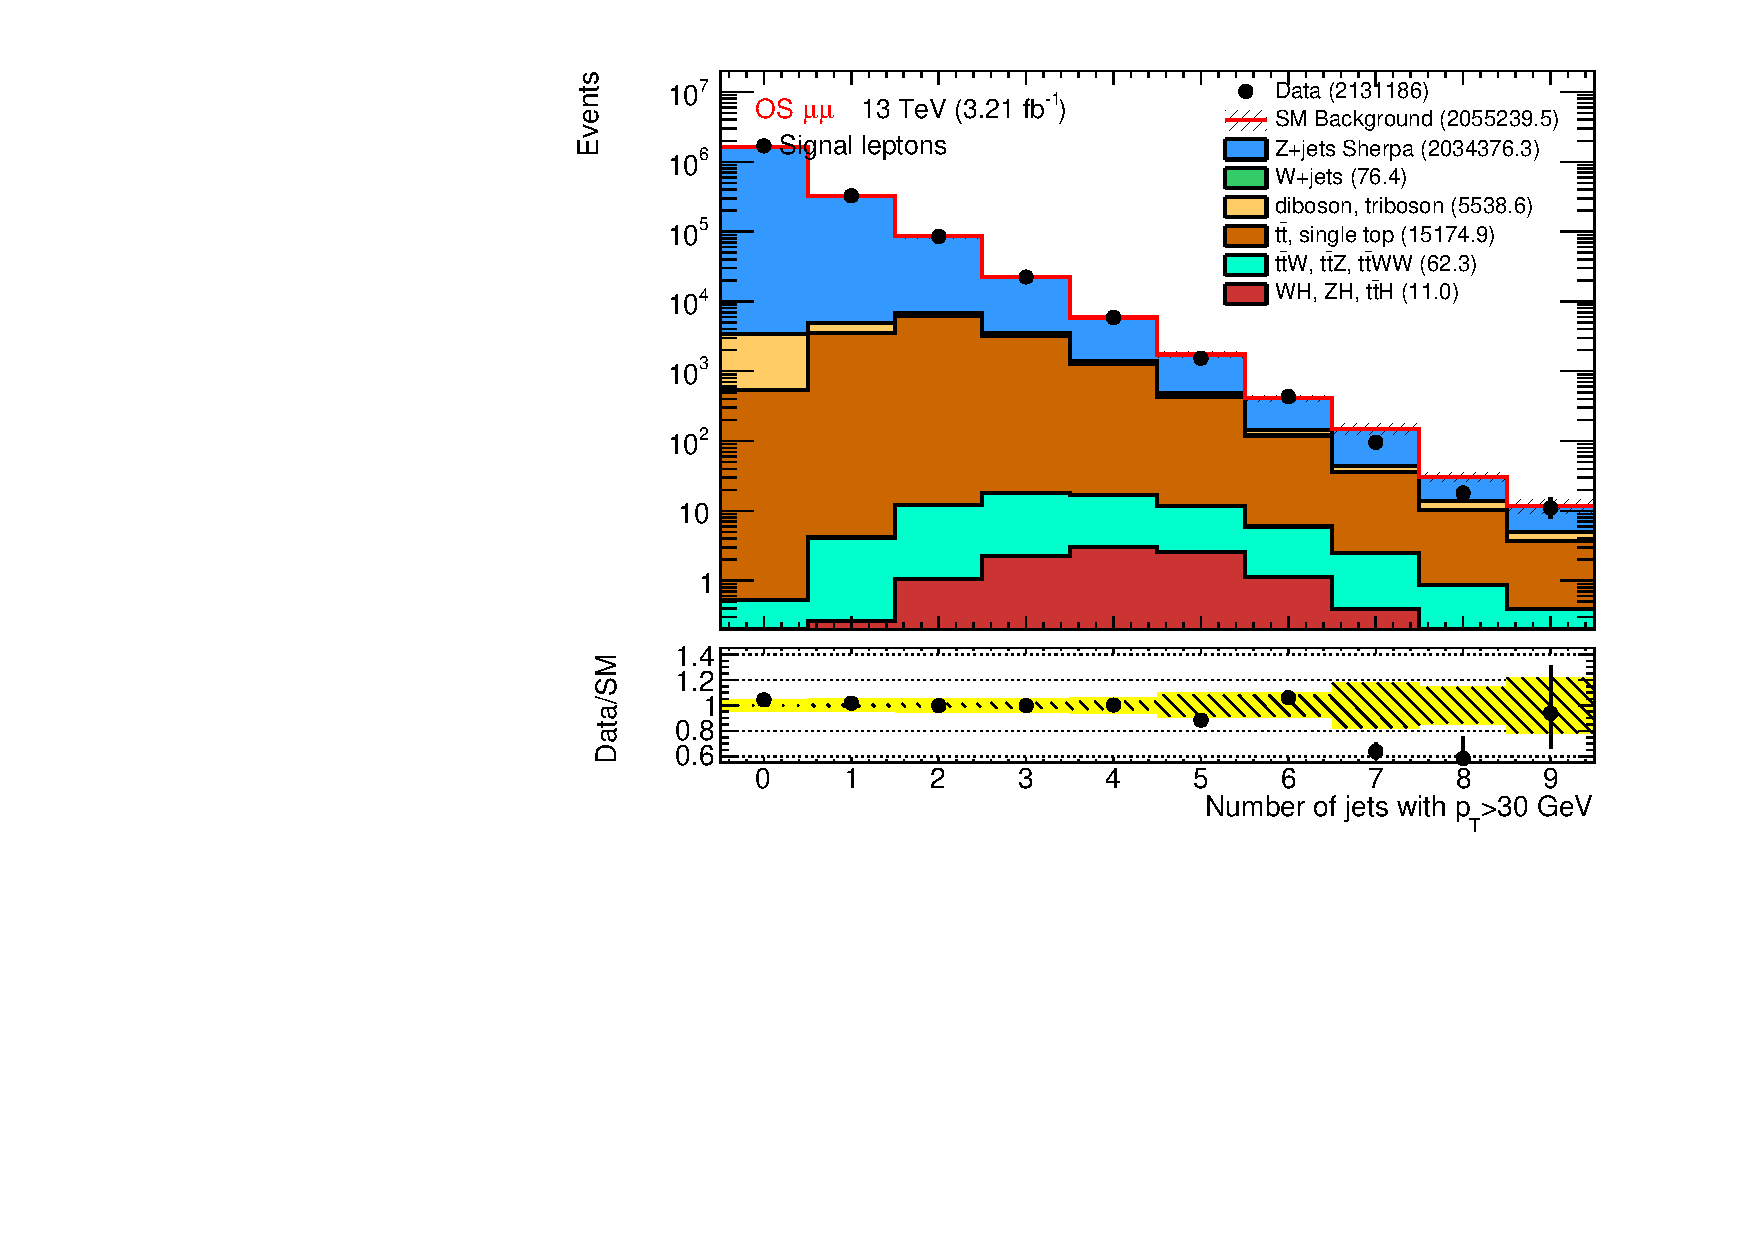
\includegraphics[width=0.45\textwidth]{DATAMC/NJET30_afterlepton_OSmm_0_physics.pdf}}
{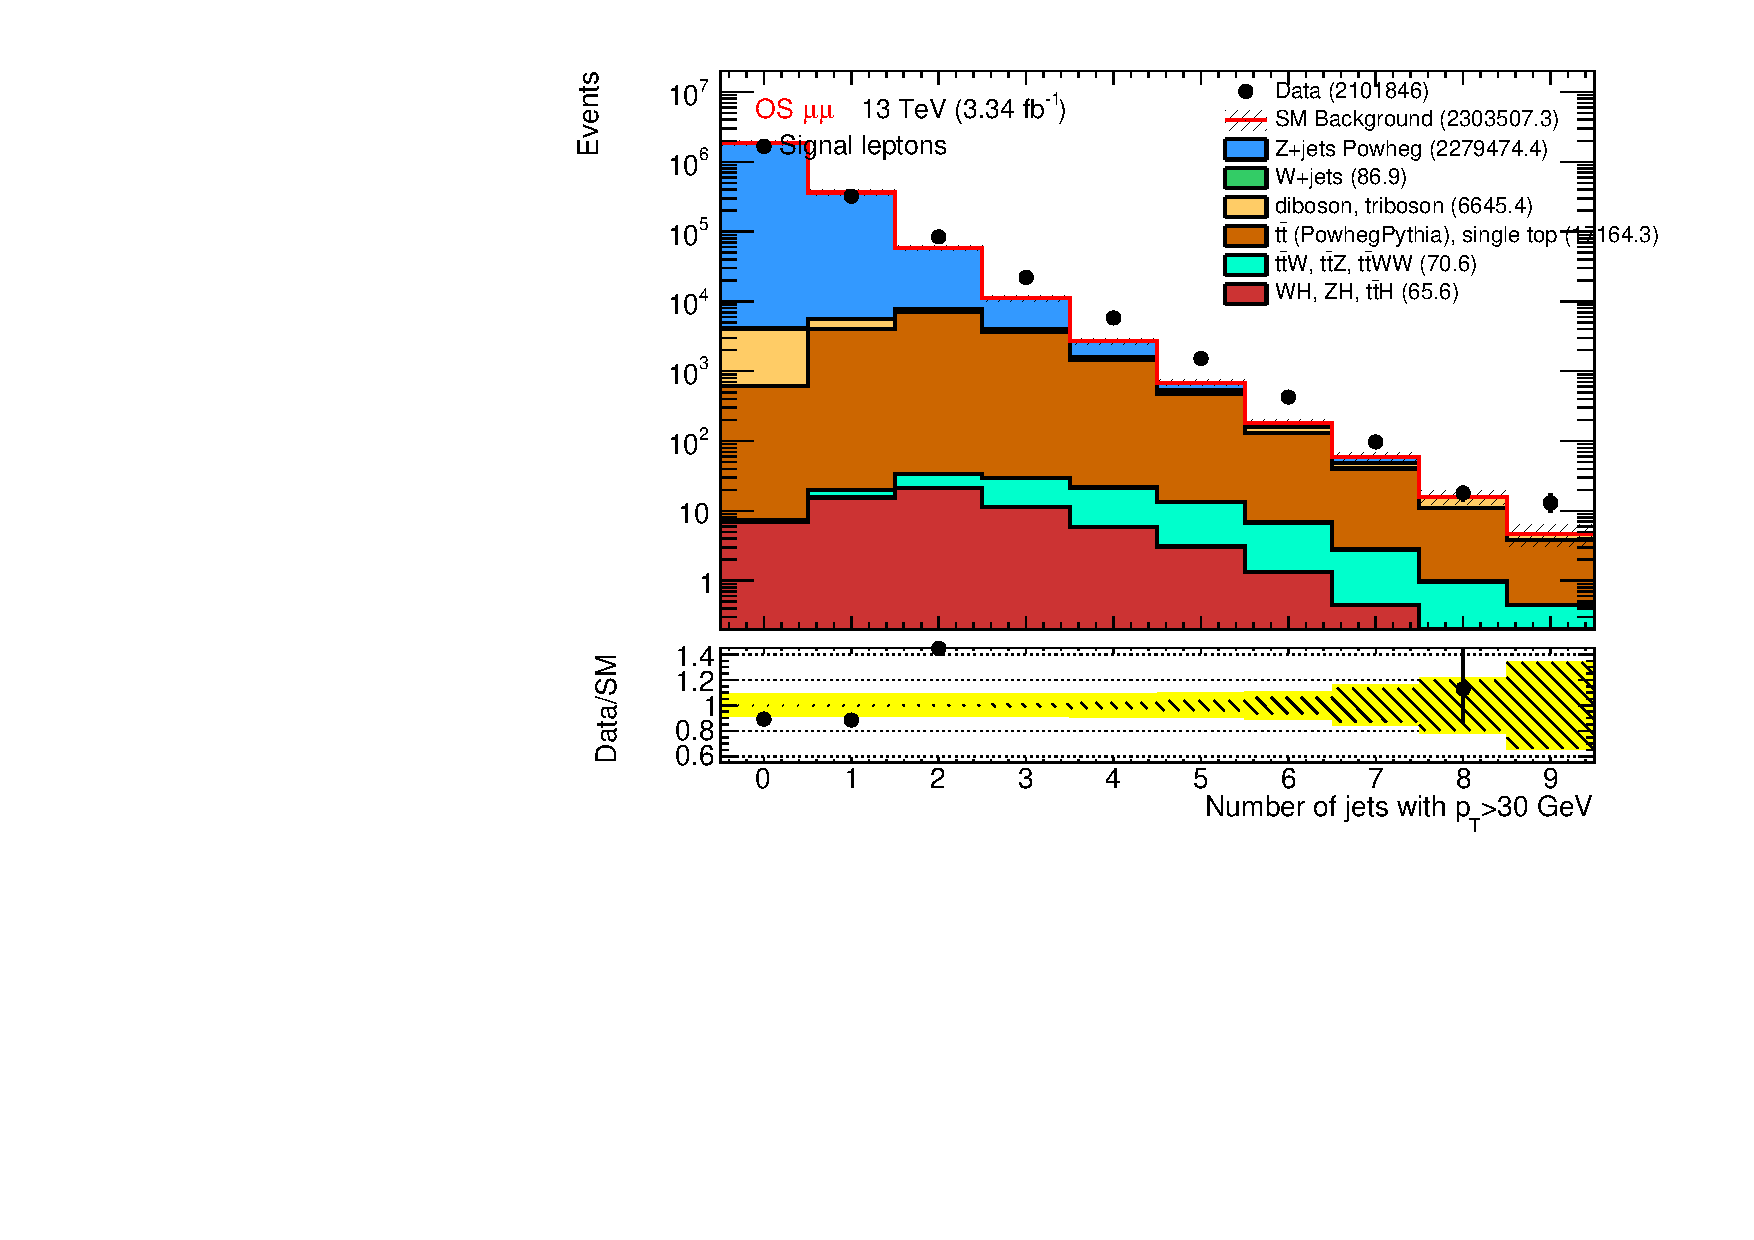
\includegraphics[width=0.45\textwidth]{DATAMC/NJET30_afterlepton_OSmm_0_physics_powheg.pdf}}
\caption{Distributions of the jet multiplicity for OS dilepton events in the $ee$ (top), $e\mu$ (middle) and $\mu\mu$ (bottom). The background contribution is taken directly from MC with no data-driven estimation of the background with fake and non-prompt leptons or charge mis-identification. Only luminosity and MC statistical uncertainties are included. The $Z$+jets background is modeled by Sherpa (left) and Powheg (right).
}
\label{fig:app_Njet_PowhegSherpa}
\end{figure}


\begin{figure}[htb!]
\centering
{\includegraphics[page=3,width=0.45\textwidth]{DATAMC/dphi.pdf}}
{\includegraphics[page=6,width=0.45\textwidth]{DATAMC/dphi.pdf}}
{\includegraphics[page=9,width=0.45\textwidth]{DATAMC/dphi.pdf}}
{\includegraphics[page=12,width=0.45\textwidth]{DATAMC/dphi.pdf}}
{\includegraphics[page=15,width=0.45\textwidth]{DATAMC/dphi.pdf}}
\caption{Distributions of $\phi(\met)$, and its difference with the $\phi$ of the two leading jets and lepton for SR1b. The background contribution is taken directly from MC with no data-driven estimation of the background with fake and non-prompt leptons or charge mis-identification. Only luminosity and MC statistical uncertainties are included.
}
\label{fig:app_Dphi_SR1b}
\end{figure}


\begin{figure}[htb!]
\centering
{\includegraphics[page=2,width=0.45\textwidth]{DATAMC/dphi.pdf}}
{\includegraphics[page=5,width=0.45\textwidth]{DATAMC/dphi.pdf}}
{\includegraphics[page=8,width=0.45\textwidth]{DATAMC/dphi.pdf}}
{\includegraphics[page=11,width=0.45\textwidth]{DATAMC/dphi.pdf}}
{\includegraphics[page=14,width=0.45\textwidth]{DATAMC/dphi.pdf}}
\caption{Distributions of $\phi(\met)$, and its difference with the $\phi$ of the two leading jets and lepton for SR0b5j. The background contribution is taken directly from MC with no data-driven estimation of the background with fake and non-prompt leptons or charge mis-identification. Only luminosity and MC statistical uncertainties are included.
}
\label{fig:app_Dphi_SR0b5j}
\end{figure}

\begin{figure}[htb!]
\centering
{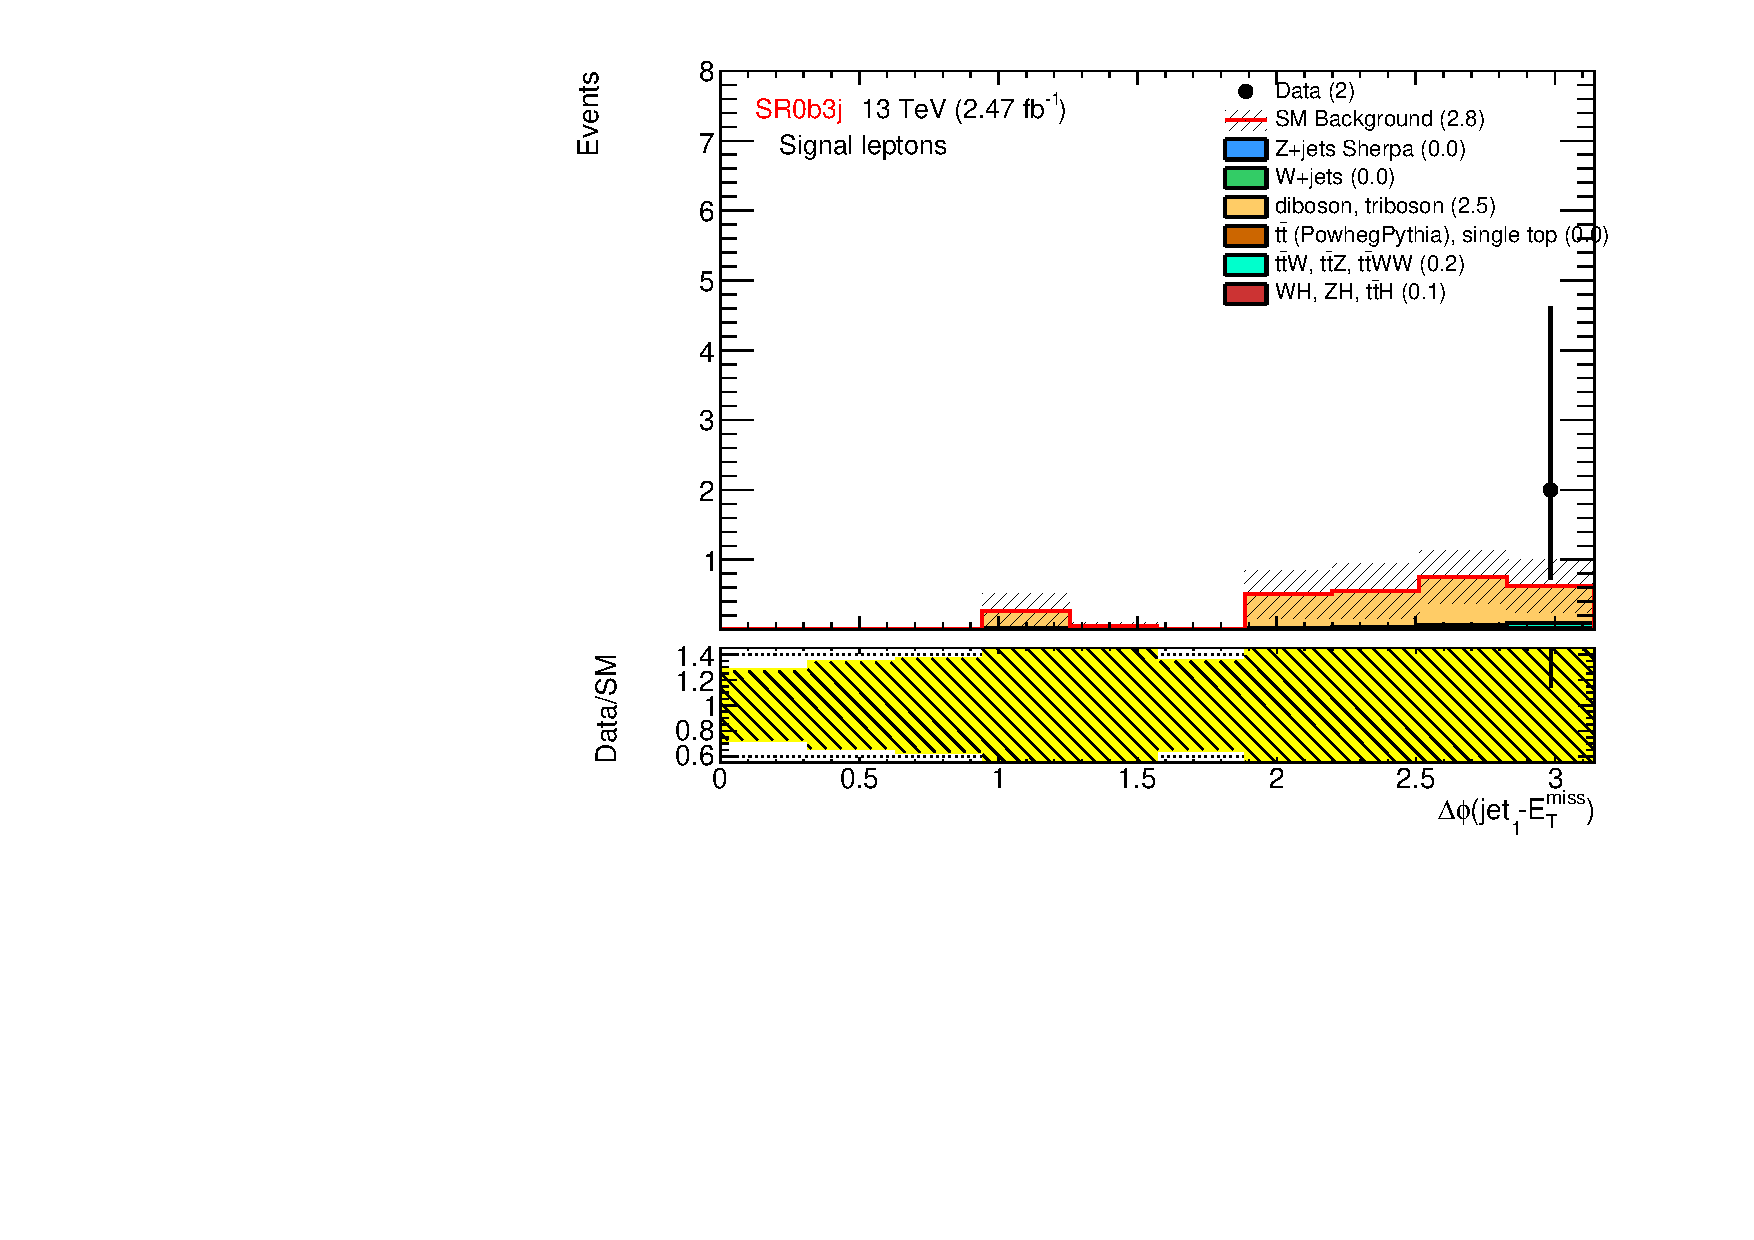
\includegraphics[page=1,width=0.45\textwidth]{DATAMC/dphi.pdf}}
{\includegraphics[page=4,width=0.45\textwidth]{DATAMC/dphi.pdf}}
{\includegraphics[page=7,width=0.45\textwidth]{DATAMC/dphi.pdf}}
{\includegraphics[page=10,width=0.45\textwidth]{DATAMC/dphi.pdf}}
{\includegraphics[page=13,width=0.45\textwidth]{DATAMC/dphi.pdf}}
\caption{Distributions of $\phi(\met)$, and its difference with the $\phi$ of the two leading jets and lepton for SR0b3j. The background contribution is taken directly from MC with no data-driven estimation of the background with fake and non-prompt leptons or charge mis-identification. Only luminosity and MC statistical uncertainties are included.
}
\label{fig:app_Dphi_SR0b5j}
\end{figure}